%\NeedsTeXFormat{LaTeX2e}[1995/12/01]

\documentclass[11pt,twoside,onecolumn,a4paper,openright,notitlepage]{book}[2001/04/21]
\usepackage[dvips]{graphicx}
\usepackage{marvosym}
\pagestyle{empty}

\usepackage{epsfig}
\usepackage{amssymb}
\usepackage{array}
\usepackage{textcomp}
\usepackage{longtable}
\usepackage[pdftex, colorlinks=true, urlcolor=black]{hyperref}

\addtolength{\hoffset}{-1.0cm}
\addtolength{\textwidth}{2.0cm}
\setlength{\oddsidemargin}{50pt}
\setlength{\evensidemargin}{50pt}

\usepackage{fancyhdr}
\pagestyle{fancy}
\renewcommand{\chaptermark}[1]{%
 \markboth{\thechapter.\ #1}{}}
%\fancyhead[LO, RE]{version 0.22 (rc1)}
\fancyhead[LE, RO]{\it Wordom User's Guide}

\fancyfoot[C]{\thepage}

\makeatletter
\def\@makeschapterhead#1{%
  \vspace*{-00\p@}%
  {\parindent \z@ \raggedright
    \normalfont
    \interlinepenalty\@M
    \Huge \bfseries  #1\par\nobreak
    \vskip 40\p@
  }}
\makeatother

\hypersetup{%
  pdfauthor={Michele Seeber},%
  pdftitle={Wordom User's Guide},%
  pdfsubject={Manual for the Wordom molecular structures and dynamics analysis program},
  pdfkeywords={wordom, molecule, dynamics, analysis}
}
\setcounter{tocdepth}{4}
\hyphenation{PROGRESSIVE mseeber}
\pdfinfo{
  /Author (Michele Seeber)
  /Title  (Wordom Users' Guide)
  /CreationDate (D:20140724180000)
  /Subject (The Users' Guide for Wordom, the friendly molecular structure analysis and manipulation tool)
  /Keywords (Wordom, molecule, analysis)
}

\begin{document}

\pagenumbering{roman}
% ##################### Ad Hoc Built Title Page ##################### %

\begin{titlepage}
\begin{center}
\rule[1cm]{15cm}{0.05cm}
%\vspace{4.0cm}
\bfseries {\huge Wordom User's Guide}\\ \vspace{0.4cm}
          {\large Version 0.23-rc1}\\ \vspace{0.2cm}
          {\large \today}
\rule[-0.5cm]{15cm}{0.051cm}

\vspace{2.25cm}

\includegraphics[scale=0.75]{images/wlogo.pdf}
\end{center}
\vspace{2.25cm}
%
\noindent\textbf{\large Developers}: Michele Seeber, Angelo Felline, Francesco Raimondi, Marco Cecchini, Simone Conti, Stefanie Muff, Ran Friedman, Francesco Rao, Gianni Settanni
\vspace{0.3cm}

\noindent\textbf{\large License}: GPL
\vspace{0.3cm}

\noindent\textbf{\large URL}: \url{http://wordom.sf.net/}
\vspace{0.3cm}

\noindent\textbf{\large Mantainer}: \href{mailto:mseeber@unimore.it}{mseeber@unimore.it}
\vspace{0.3cm}

\noindent\textbf{\large Description}: Wordom is a command line tool written to deal with structure and molecular dynamics files. It allows to access the information in such files, convert it, and analyse it. New analysis modules can be easily added.
\end{titlepage}
\thispagestyle{plain}
\cleardoublepage

% ##################### ####################### ##################### %
\tableofcontents
\clearpage

\pagenumbering{arabic}

% ##################### General Intro ##################### %

\chapter{Introduction}
%\addcontentsline{toc}{chapter}{Introduction}

Wordom is a (simple) command line utility conceived to spare the user some time in manipulating and converting pdb, crd, dcd, xtc and xyz files. Wordom is also a versatile program for a broad range of analysis of molecular dynamics trajectories. As a plus, it's easy to use Wordom both from the command line and in shell scripts.\\
Due to its simplicity, it is very easy and straightforward to add your own analysis module. Basically, all you have to do is write the algorithm. The data are made available by the existing wordom i/o modules.

\section{Contacting the authors}
Wordom has been developed by Michele Seeber with the crucial help of A. Felline, F. Raimondi, M. Cecchini, S. Conti, S. Muff, R. Friedman, F. Rao and G. Settanni.\\
For bug-alerts or questions about Wordom you can contact him at \href{mailto:mseeber@unimore.it}{mseeber@gmail.com}. Although Wordom development and maintenance are not his only (nor main) activity he will do his best to answer and/or help. Wordom is in more or less constant development, so bugs may appear and the contribution of users is highly regarded as a polishing tool.


\section{Citation Reference}
If you use Wordom in your work, we would like you to cite the relevant Wordom paper(s)\cite{mseeber:wordom,mseeber:wordom2}:
\begin{center}
M. Seeber, M. Cecchini, G. Settanni, F. Rao and A. Caflisch; \\
\emph{Wordom: a program for efficient analysis of molecular dynamics simulations};\\
 Bioinformatics (2007); 23(19), 2625-2627; doi: 10.1093/bioinformatics/btm378
\end{center}

\begin{center}
M. Seeber, A. Felline, F. Raimondi, S. Muff, \\Ran Friedman, F. Rao, A. Caflisch and F. Fanelli; \\
\emph{ Wordom: a user-friendly program for the analysis of molecular\\structures, trajectories, and free energy surfaces};\\
 J. Comp. Chem. (2011); 32, 1183-1194; doi:10.1002/jcc.21688
\end{center}

along with any paper(s) regarding the particular module you are using (see relevant section(s)).

\section{Acknowledgments}
Wordom has been developed with the help of a number of people who contributed with requests, suggestions, bits of code, extensive testing and debugging and so forth. Among others we would like to mention and thank N. Majeux, A. Cavalli, P. Kolb, D. West, Y. Valentini and A. Vitalis.

\section{Copyright and Disclaimer Notices}
Wordom is Copyright \copyright{} 2003-2014 the University of Modena and Reggio Emilia and the University of Zurich.


Wordom is free software; you can redistribute it and/or modify
it under the terms of the GNU General Public License as published by
the Free Software Foundation; either version 3 of the License, or
(at your option) any later version.

Wordom is distributed in the hope that it will be useful,
but WITHOUT ANY WARRANTY; without even the implied warranty of
MERCHANTABILITY or FITNESS FOR A PARTICULAR PURPOSE.  See the
GNU General Public License for more details.

You should have received a copy of the GNU General Public License
along with Wordom.  If not, see \url{http://www.gnu.org/licenses/}

% ##################### installation ##################### %

\chapter{Installation}
%\addcontentsline{toc}{chapter}{Installation}

Wordom is distributed as binaries for some popular operating systems (OS), such as commonly used linux flavours, and source code which can be compiled on other platforms.\\
Both binaries and source code can be downloaded at the website:\\
\url{http://www.wordom.sf.net}

Compilation requires a C compiler, the \emph{make} and \emph{cmake} programs and the BLAS plus LAPACK libraries (Basic Linear Algebra System and Linear Algebra PACKage). These are
light requirements, since free C compilers are widely available and
\emph{make}, \emph{cmake} and BLAS/LAPACK are fairly ubiquitous.\\

To compile, just get in the \emph{build} directory and issue the commands:\\

\begin{verbatim}
 cmake ..
 make
\end{verbatim}

cmake generates an appropriate makefile for your system: just check for any error/warning message. Missing libraries might prevent compilation or force a compilation without some modules. If all goes well a binary will be built in the build directory.

Wordom can be sometimes be compiled on MacOSX, but we encourage you to check the first results twice before trusting them. No serious attempts to compile wordom on windows have been recently made - which doesn't mean that it is impossible.

\section{Note for Gromacs Users}
Wordom performance while running analysis on large xtc files is often disappointing, partly due to the difficulty in randomly accessing frames in xtc files. You might be faster by simply converting your xtc file to a dcd and running your analysis on the latter. Of course, this is especially true if your have multiple analyses to run.\\

%Hopefully, things will be smoother with the next version(s) of Gromacs and Wordom.

% ##################### Files and Selections ##################### %

\chapter{Files and Selections}
%\addcontentsline{toc}{chapter}{Files and Selections}

\section{File Formats}
Wordom can deal with pdb and crd as structure files, \emph{i.e.} containing both a coordinate set and structure information (residues, atoms etc). Informations about these file formats can be found, respectively, at the Protein Data Bank:\\ http://www.wwpdb.org/docs.html\\
and in the Charmm documentation:\\ http://www.charmm.org/document/Charmm/c32b2/io.html\#Coordinate\\
Wordom can read trajectories in the dcd and xtc formats. Dcd is the native format for the Charmm program. NAMD$^{\tiny \copyright{}}$ uses a very similar format that can be read by Wordom. These files only contain coordinate sets (called ``frames''), so that, when dealing with them, it is often necessary to also load a structure file.\\
Wordom can also deal with .xtc files:\\
http://www.gromacs.org/documentation/reference/online/xtc.html \\
However, you should be aware that not all functions are currently working with xtc files, and that wordom does not (yet) deal with some kind of PBC as implemented in Gromacs. The \emph{few} modules that understand and use PBC data require a rectangular box (the easiest to deal with).

XYZ files, ie ASCII files with only the coordinates listed, are also sporadically used: noticeably, they can be produced by wordom in order to make a coordinate set (or a number of coordinate sets, such as a whole trajectory) easily available.

In this manual, structure files such as pdb and crd files will be collectively referred to as \emph{mol}, while trajectory files such as dcd an xtc will be collectively referred to as \emph{trj}
%you should be aware of the following. First, not all functions work with xtc. Second, periodicity is not taken into account in Wordom. The only exception is that when converting DCD to XTC, Wordom will read the CRYST1 identifiers from the attached PDB file and store them as box vectors in the XTC. This will only make sense if the DCD file contains constant volume data.

\section{Selections}

For analysis and manipulation it is often necessary to select a subset of atoms. Wordom has a selection mechanism which employs a string structured as follows:
\begin{verbatim}
/chainID/segname/resnumber/atomtype
\end{verbatim}
{\bf Note:} segname is the $12^{th}$ field in the pdb ($3^{rd}$ after coordinates) and $8^{th}$ in the crd ($1^{st}$ after coordinates). It is a 4 letter field, not to be confused with the chain (single character) field found after the residue type in the pdb ($5^{th}$ field). No chain is present in crd files.

\subsection{Wild Cards}
Wild cards such as * (any number of any character), ? (any single character), [abc] (any single character among a, b and c) and [!abc] (any single character except a, b and c) are supported.
\begin{verbatim}
/*/*/*/CA                 -> all alpha carbons
/*/MOL1/*/*               -> all atoms in segment MOL1
/*/MOL?/*/*               -> all atoms in MOL1, MOL2, MOLA etc.
/*/*/*/C[AB]              -> all alpha and beta carbons
\end{verbatim}
{\bf Note:} please take care to protect the selection string with quotes whenever you are submitting a selection with special characters (\emph{eg}: *, ?, (, )) on the command line, since most shells will try to interpret them.

\subsection{Short Forms}
Wordom accepts selection strings with fewer than 4 fields or with empty fields. Wordom takes the rightmost field to indicate atoms, the one to its left residues etc. Empty or missing fields are taken as \emph{*}.
\begin{verbatim}
/CA       -> /*/*/*/CA    -> all alpha carbons
/         -> /*/*/*/*     -> all atoms
/10/CA    -> /*/*/10/CA   -> C-alpha in residue 10 (all segments/chains)
/A///CA   -> /A/*/*/CA    -> alpha carbons in chain A
\end{verbatim}

\subsection{Pattern Matching}
Moreover, Wordom selection supports ksh-style pattern matching, such as:
\begin{itemize}
\item ?(pattern-list) $\to$ The pattern matches if zero or one occurrences of any of the patterns in the pattern-list allow matching the input string.
\item *(pattern-list) $\to$ The pattern matches if zero or more occurrences of any of the patterns in the pattern-list allow matching the input string.
\item +(pattern-list) $\to$ The pattern matches if one or more occurrences of any of the patterns in the pattern-list allow matching the input string.
\item @(pattern-list) $\to$ The pattern matches if exactly one occurrence of any of the patterns in the pattern-list allows matching the input string.
\item !(pattern-list) $\to$ The pattern matches if the input string cannot be matched with any of the patterns in the pattern-list. 
\end{itemize}

Where pattern-list is a $|$ (pipe) separated list of patterns. A dash can be used to indicate a range of values in the residue number

\begin{verbatim}
/@(CA|C|N)                -> backbone atoms
/!(CA|C|N|O|H|OT1|OT2)    -> non-backbone atoms
/MOL1/@(1|3|5)/*          -> residues 1, 3 and 5 of segment MOL1
/MOL1/@(1-5)/*            -> residues 1 to 5 of segment MOL1
/MOL1/@(1-5|10)/*         -> redidues 1 to 5 and 10 of segment MOL1
\end{verbatim}

\subsection{Add/Del}
An additional way to select ensembles of atoms is to use the \emph{add} and \emph{del} keywords. These are processed strictly from left to right, no parentheses allowed:

\begin{verbatim}
/MOL1/@(1-5)/*; add /MOL2/@(3-6)/*; del /MOL2/4/CA
\end{verbatim}

\subsection{\emph{within} selection tool}
It is possible to select all atoms that are found within a given distance of a selection. The syntax to select any atom within 5 \AA{} of any atom of residues 23 to 25 of segment MOL1 is:
\begin{verbatim}
/MOL1/@(23-25)/*[5]
\end{verbatim}
Some modules are able (or will be) to re-compute the selection along the trajectory, since this mechanism allows it to change with the atoms moving around, but it is not standard behaviour - \emph{ie} it will not happen unless you specify it, except in the ``within'' module.

\subsection{Index file}
Wordom can also get the selected atoms from an index file, where the desired atoms'ID numbers are listed (one number per line). Since Wordom can also \emph{produce} such an index file (with the \hyperref[csele]{-checksele} option), this allows to combine different selections in ways not possible with a single selection string.

\begin{verbatim}
wordom -checksele "/MOL1/*/CA" -imol reference.pdb > sele1.txt
wordom -checksele "/MOL2//N" -imol reference.pdb >> sele1.txt
sort -n sele1.txt > sele2.txt
wordom -sele sele2.txt -imol reference.pdb
\end{verbatim}

\subsection{Checksele\label{csele}}
The \emph{-checksele} command prints to the screen the selection, the number of selected atoms and the atom number for each selected atom. This is a very important tool that allows you both to use the \emph{index} feature described above and, crucially, to check the atoms that wordom is actually using in your manipulation/calculation in case something doesn't work as expected. Ideally, a quick check with \emph{checksele} is always advisable.
\begin{verbatim}
bash > wordom -checksele "/@(1-5)/CA" -imol 1CRN.pdb
#N of selected atoms (/@(1-5)/CA): 5
2
9
16
22
28

\end{verbatim}

%\subsection{What Else?}
%At this stage, the selection routine is very simple and reasonably effective, but not particularly flexible or powerful. We are aware of that. Work on it is not over, though it is not on top of the priority list.

% ##################### Coordinates  Manipulation ##################### %

\chapter{Coordinates  Manipulation}
%\addcontentsline{toc}{chapter}{Coordinates  Manipulation}

These are the basic Wordom capabilities. You can use them to convert your coordinate files in the way better suited to your needs.\\
In the following examples, valid trj files are dcd and xtc files and valid structure files are pdb and crd files, unless otherwise stated.\\
The general syntax is organized as follows:
\begin{verbatim}
-imol    input structure file
-omol    output structure file
-itrj    input trj file
-otrj    output trj file
-sele    selection string or index file
\end{verbatim}

\section{Extraction of a trj frame to a mol file}
\textbf{\large Options}:
\begin{verbatim}
-F       frame_number
-itrj    trj file
-imol    input structure file
-omol    output structure file
-sele    selestring (optional)
\end{verbatim}
Frame number frame\_number is read from the trj file and written to output structure file. The input structure file is needed as a reference since trjs do not have any information regarding structure. If the (optional) \emph{-sele} option is used, a mol file with only the selected atoms will be created\\

\textbf{\large Example}:
\begin{verbatim}
wordom -f 35 -itrj trajectory.dcd -imol reference.pdb -omol frame35.pdb
\end{verbatim}
%\pagebreak
%
\section{Extraction of several trj frames to mol files}
\textbf{\large Options}:
\begin{verbatim}
-F       frame_number list file
-itrj    trj file
-imol    input structure file
-omol    output structure file
-sele    selestring (optional)
\end{verbatim}
All frames listed in the frame list file are read from the trj file and written to output structure files. The basename for the output files is taken from the omol option, plus a number indicating the frame number. A extension-less name works best. If the keyword \emph{all} is used, all frames are used. If the keyword \emph{range} is used together with \emph{-beg} and \emph{-end}, all frames ranging from beg to end (included) will be extracted. The input structure file is needed as a reference since trjs do not have any information regarding structure. If the (optional) \emph{-sele} option is used, mol files with only the selected atoms will be created\\

\textbf{\large Example}:
\begin{verbatim}
wordom -F framelist.txt -itrj trajectory.dcd -imol reference.pdb -omol frame
\end{verbatim}
%\pagebreak
%
\section{Extraction of a frames series from a trj to a trj}
\textbf{\large Options}:
\begin{verbatim}
-F       framelistfile
-itrj    inTRJfile
-otrj    outTRJfile     
-imol    input structure file (optional)
-sele    selestring (optional)
\end{verbatim}
Several frames, listed (one frame per line) in a specified file are read from a trj and written to a newly created trj. If the keyword \emph{all} is used, all frames are used. If the keyword \emph{range} is used together with \emph{-beg} and \emph{-end}, all frames ranging from beg to end (included) will be extracted.\\
If a reference mol and a selection are specified, only the selected atoms will be part of the new trajectory. In combination with the \emph{-F all} feature, this is a way to isolate part of your system.\\

\textbf{\large Example}:
\begin{verbatim}
wordom -F framelist.txt -itrj orig_trj.dcd -otrj newtray.dcd
wordom -F all -itrj orig_trj.dcd -imol file.pdb -sele "/A/*/*" -otrj newtray.dcd
wordom -F range -beg 101 -end 200 -itrj orig_trj.dcd -otrj newtray.dcd
\end{verbatim}
%\pagebreak
%
\section{Merging of trjs into a single trj}
%\subsection{Using a list}
\textbf{\large Options}:
\begin{verbatim}
-itrj    trjlistfile
-otrj    TRJfile     
-skip    skipstep
\end{verbatim}
The trj files listed in a specified file (one filename per line) are merged into a newly created trj file. Optionally, a skip step can be specified and only one every skipstep frames are considered.\\

\textbf{\large Example}:
\begin{verbatim}
wordom -itrj trjlist.txt -otrj newtray.dcd
\end{verbatim}
%\subsection{Using a common basename}
%\textbf{\large Options}:
%\begin{verbatim}
%-m       basename
%-beg     firstdcd_number
%-end     lastdcd_number
%otrj    outDCDname
%skip    skipstep
%\end{verbatim}
%everal dcd files with a common basename and a numerical, progressive suffix \basenamenumber.dcd) are merged and written to a newly created dcd. Optionally, a skip step can be specified and only one every skipstep frames are considered.\\
%
%\textbf{\large Example}:
%\begin{verbatim}
%wordom -m mytrj -beg 1 -end 10000 -otrj newtrj.dcd -skip 100
%\end{verbatim}
%\pagebreak
%
\section{Appending a trj to another trj}
\textbf{\large Options}:
\begin{verbatim}
-atrj    TRJ1
-otrj    TRJ2     
\end{verbatim}
TRJ1 is appended to TRJ2, \emph{i.e} all frames of TRJ1 are placed at the bottom of TRJ2, whose frame number is raised accordingly. Both TRJs must have the same number of atoms. Header values such as timestep, skipstep and the like are kept in the original target trajectory\\

\textbf{\large Example}:
\begin{verbatim}
wordom -atrj trajpiece.dcd -otrj wholetraj.dcd
\end{verbatim}
%\pagebreak
%
\section{Appending a structure's coordinates to a trj}
\textbf{\large Options}:
\begin{verbatim}
-amol    MOLfile
-otrj    TRJfile     
\end{verbatim}
MOL is appended to TRJ, \emph{i.e} the coordinate set from the structure file (be it a pdb or a crd) is placed at the bottom of TRJ, whose frame number is raised accordingly. \\

\textbf{\large Example}:
\begin{verbatim}
wordom -amol mymolecule.pdb -otrj traj.dcd
\end{verbatim}
%\pagebreak
%
\section{Convertion of a structure to a 1-frame trj}
\textbf{\large Options}:
\begin{verbatim}
-mono
-imol    MOLfile
-otrj    TRJfile     
\end{verbatim}
The ``mono'' flag activates the module. PDB or CRD is converted to a TRJ, \emph{i.e} a trajectory file with a single coordinate set (frame) taken from the structure file. The header of the TRJ is correct, but values for timestep and the like are arbitrary.\\

\textbf{\large Example}:
\begin{verbatim}
wordom -mono -imol mymolecule.pdb -otrj smalltraj.dcd
\end{verbatim}
%\pagebreak
%
\section{Convertion of file formats}
\textbf{\large Options}:
\begin{verbatim}
-conv
-imol    MOL1file
-omol    MOL2file
-itrj    TRJ1file
-otrj    TRJ2file
-sele    selestring (optional)
\end{verbatim}
The -conv flag activates the file conversion, which works both between mol and trj formats. Dcd to xtc conversion also requires a reference pdb. The box size and structure are taken from the CRYT1 section of the pdb file, and is not updated. When starting from a mol file, if the (optional) \emph{-sele} option is used, a mol file with only the selected atoms will be created\\
In case the starting mol file (pdb format) has alternate locations, more than 1 output file will be created, one for each flag found in the altloc field. Thus outfile\_A.pdb, outfile\_B.pdb etc will be created. There is no way (at the moment) to choose the locations - all A locations will end up in file\_A, all B in file\_B. \\

\textbf{\large Example}:
\begin{verbatim}
wordom -conv -imol mymolecule.pdb -omol mymolecule.crd
wordom -conv -imol mymolecule.pdb -sele "/A/@(20-100)/*" -omol mymolecule.crd
wordom -conv -itrj mytrj.dcd -imol mymolecule.pdb -otrj mytrj.xtc
wordom -conv -itrj mytrj.xtc -otrj mytrj.dcd
\end{verbatim}
%\pagebreak
%
\section{Convertion of a trj to a concatenated xyz}
\textbf{\large Options}:
\begin{verbatim}
-conv
-itrj    TRJfile
-omol    XYZfile
-sele    selestring (optional)
\end{verbatim}
A trj file is converted to an ASCII file with xyz coordinates of each (selected) atom on a line. Frames are separated by a line reporting the frame number as XYZ framenumber. Selection is possible (a structure mol file is then needed).\\

\textbf{\large Example}:
\begin{verbatim}
wordom -conv -imol structure.pdb -itrj mytray.dcd -omol file.xyz -sele "/CA"
\end{verbatim}
%\pagebreak
%
\section{Showing a trj's headers}
\textbf{\large Options}:
\begin{verbatim}
-head    TRJfile
\end{verbatim}
A TRJ's headers are read and printed out. This gives information about the size of the system, the lenght of the simulation and some simulation setup. In Wordom-generated TRJ this settings are arbitrary and do not have any meaning. it also gives the ``claimed'' number fo frames versus the ``real'' number of frames, so that it is possible to know how far the computation has been running if dealing with a TRJ that is being produced by an ongoing simulation.\\

\textbf{\large Example}:
\begin{verbatim}
wordom -head mytray.dcd
\end{verbatim}
%\pagebreak
%
\section{Modifying a dcd's headers}
\textbf{\large Options}:
\begin{verbatim}
-mod     flag=value
-itrj    DCDfile
\end{verbatim}
A DCD's headers can be modified. This might be necessary if some setting's values have not been conserved. This is a peculiar feature, not widely used or (in general) particularly useful. There shouldn't be many occasions where you will need it. {\bf Note:} the submitted dcd file is modified! A backup is advisable.\\

\textbf{\large Example}:
\begin{verbatim}
wordom -mod nframe=5000 -itrj mytray.dcd
wordom -mod begstep=1 -itrj mytray.dcd
wordom -mod numstep=5000 -itrj mytray.dcd
wordom -mod skpstp=5000 -itrj mytray.dcd
wordom -mod tmstp=0.2 -itrj mytray.dcd
\end{verbatim}
%\pagebreak
%
\section{Summing several trjs to a single trj}
\textbf{\large Options}:
\begin{verbatim}
-S       trjlistfile
-imol    MOLfile
-otrj    TRJfile     
-sele    selectionstring
\end{verbatim}
The trj files listed in a specified file (one filename per line) are summed into a newly created trj. That is, every frame is given by the sum of the differences of each listed TRJ's corresponding frame with respect to the reference structure, added to the reference structure itself. This is used after a PCA run (and a \emph{projection} module run), to sum the projections along different eigenvectors to a single trajectory. The \emph{-sele} argument is NOT optional and, at the moment, MUST be equal to the selection given in the PCA (and \emph{projection}) run.\\

\textbf{\large Example}:
\begin{verbatim}
wordom -S trjlist.txt -imol reference.pdb -otrj newtray.dcd -sele "/*/*/CA"
\end{verbatim}
%\pagebreak
%
\section{Average over a trj}
\textbf{\large Options}:
\begin{verbatim}
-avg
-imol    MOLfile
-itrj    TRJfile     
-omol    averagePDB
\end{verbatim}
An average is computed on all the frames in a TRJ file and written to a MOL file\\

\textbf{\large Example}:
\begin{verbatim}
wordom -avg -imol mypdb.pdb -itrj mytrj.dcd -omol average.pdb
\end{verbatim}
%

% ##################### Trajectory Analyses ##################### %

\chapter{Trajectory Analyses}
%\addcontentsline{toc}{chapter}{Trajectory Analyses}

Wordom can run analysis along a trajectory. All these analysis modules need a structure file (pdb or crd) as a reference and a trajectory file (dcd or xtc) to provide the coordinate sets (it is possible to provide a list of trj files). An input file is also required, in which the required module is to be specified along with the appropriate options.

\begin{verbatim}
wordom -iA analysis.inp -imol file.pdb -itrj file.dcd
\end{verbatim}

Or, as an alternative, the command line can be used. Here, the desired module has to be passed as an argument of the -ia option, while all parameters for the module itself must be passed just like they would appear in the input file, ie with leading double hyphen -{}- and in uppercase. Fields like selections must also be appropriately shielded from the shell :

\begin{verbatim}
wordom -ia rmsd --TITLE rmsd1 --SELE "/CA" -imol file.pdb -itrj file.dcd
\end{verbatim}

The \emph{-itrj} flag also accepts a list of trj files (-itrj list.txt), with one trj filename per line. Wordom takes files ending with .txt as lists and behaves accordingly. The list can also list mol (\emph{ie} pdb or crd) files, but file format has to be homogeneous in the list.

\begin{verbatim}
wordom -iA analysis.inp -imol file.pdb -itrj trjlist.txt
\end{verbatim}

Last but not least wordom can run an analysis on a subset of frames. It is possibile to specify the first frame to consider (-beg), the last one (-end), a skip step (-skip) or give a list of frames to consider (-F filename.txt ; one frame number per line).\\

In case a mol file (pdb format) with alternate atom locations is use as reference (this is a weird case since most of the times we should deal with simulations output, which do not have altlocs) the first location found is used for all atoms.\\

\section{General Notes}
\subsection{Input Files}
The input file begins with the ``BEGIN modulename'' flag that call the desired module, and ends with the ``END'' flag.\\
The ``-{}-TITLE title1'' flag allows you to give a title (here \emph{title1}): this will be written in the appropriate column of the output time series and/or used to name extra output files (clustering module, pca module).\\
Output is, unless specified, a time-series of the required parameter computed over the trajectory. Standard output (hence \emph{stdout}) is to the terminal, unless the -otxt outfile.txt option is used (results written to outfile.txt).

Wordom can run more than one analysis at once, so it is possible to write an input files where different modules are called - or the same module is called with different parameters. Keep in mind, however, that if a module works on the results of another analysis (such as PCA projections working with PCA results or 2-pass clustering), you have to run wordom twice with separate input files - each wordom run accounts for a single processing run along the trajectory.

Details for each module's input file are given in the module's section of the User Guide.

\subsection{Periodic Boundary Conditions (PBC)}
Wordom can only deal with \emph{cubic} PBC, which are not actually cubic since the lenght of each side can be different. This should be fine for most situations, since when employing non-cubic PBC (to minimize the number of water molecules) the system is usually coherent and interactions between the images are not what the user wants to consider (centering of the system when employing non-cubic boxes is thus necessary). When such interactions are under scrutiny (aggregation simulations and the like) a cubic box is perfectly suitable, since other shapes do not offer more efficiency. This is a general rule and we are sure there are exceptions. Use of wordom in such cases is still possible but extra care must be taken to avoid artifacts and results should always be checked thrice.\\
As a general rule, be extremely wary when working with wordom and PBC trajectories, and keep in mind all possible implications. As a specific rule, avoid mixing gromacs xtc files, PBC and wordom.\\
Some modules do not even support cubic PBC - starting from the assumption that the property in case is typically computed on a coherent system (\emph{ie} centered systems not crossing boundaries). Check the relevant sections to check each module's behaviour.

\subsection{Threading}
Some modules are now able to run in threads using the -nt option (number of threads). As a general guideline, those modules which output results as a time series along the trajectory are trivially threaded in that the frames are distributed among the threads and results are collected and printed out together. The results and speed are not different from what could be had by manually simultaneaously running \emph{nc} instances of wordom on different chunks of trajectory and then joining the pieces, but the process is transparent to the user and faster than running in single-thread mode - especially in those module where each frame takes some time to be processed. Thus, modules like secondary structure assignment or surface computation can greatly benefit from threading, while simpler, faster modules, where data-access is the bottleneck, might not show a real improvement.\\
Threading is also implemented for the clustering module (not all algorithms) where the bulk of the job is not along the trajectory, but the threading is then called \emph{inside} the module (see specific section).
\\
%\pagebreak
\clearpage{}

\section{Distances (DISTANCE)}
This module computes the distance between two atoms or group of atoms. In case more than one atom is selected the geometric center is considered. In the presence of a periodic boundary sysmte, though, the center will be computed without considering the PBC, so care must be taken to ensure that all the selection is actually in the same cell. If the option MASS is used, the center-of-mass will be used. In this case, masses for each atoms should be reported in the $\beta{}$-factor field (or wmain if dealing with crd). Also, it is possible to compute more than one distance inside the same BEGIN/END group, splitting the different distance selection with a TITLE. This may be (very slightly) faster than using separate BEGIN/END grouping, but the MASS setting is shared among all distances computed in a BEGIN/END section.\\

\textbf{\large Sample Input}:
\begin{verbatim}
BEGIN distance
--TITLE thisdist
--SELE /A/12/CA : /A/26/CA
--TITLE moredist
--SELE /A/13/CA : /A/25/CA
--TITLE scdist
--SELE /A/14/!(CA|N|O|C|HN) : /A/24/!(CA|N|O|C|HN)
END
BEGIN
--TITLE scdist2
--MASS 1
--SELE /A/14/!(CA|N|O|C|HN) : /A/24/!(CA|N|O|C|HN)
END
\end{verbatim}

\textbf{\large Sample Command Line}:\\\\
%\begin{verbatim}
\textsf{\large wordom -ia distance -{}-TITLE distA -{}-SELE "/A/1/N : /A/8/O" -imol file.pdb -itrj file.trj}
%\end{verbatim}

%\pagebreak
\clearpage{}

\section{Contacts (CONTACTS)}
This module checks whether two atoms or group of atoms are within a user-defined cutoff (in \AA{}ngstrom). In case more than one atom is selected the geometric center is considered. If the MASS option is used, center-of-mass is used. In this case, masses for each atoms should be reported in the $\beta{}$-factor field (or wmain if dealing with crd). Also, it is possible to compute more than one contacts inside the same BEGIN/END group, splitting the different contact selection with a TITLE. See also the distance module for details.\\

\textbf{\large Sample Input}:
\begin{verbatim}
BEGIN contacts
--TITLE contact1
--SELE /A/12/CA : /A/26/CA : 4
--TITLE contact2
--SELE /A/13/CA : /A/25/CA : 4
--SELE /A/12/CA : /A/26/CA : 4
--SELE /A/11/CA : /A/27/CA : 4
--TITLE sc-cont
--SELE /A/14/!(CA|N|O|C|HN) : /A/24/!(CA|N|O|C|HN) : 4
END
\end{verbatim}

\textbf{\large Sample Command Line}:\\\\
%\begin{verbatim}
\textsf{\large wordom -ia contacts -{}-TITLE cont1 -{}-SELE "/A/14/!(CA$\mid$N$\mid{}$O$\mid{}$C$\mid{}$HN) : /A/24/!(CA$\mid{}$N$\mid{}$O$\mid{}$C$\mid{}$HN) : 4" -imol file.pdb -itrj file.trj}
%\end{verbatim}

%\pagebreak[4]
\clearpage{}

\section{Angles (ANGLE)}
This module computes the angle between three selected atoms. The atoms are selected with three separated selection strings, each of which must select one and only one atom. At the moment, periodic boundary conditions are unaccounted for in this module.\\

\textbf{\large Sample Input}:
\begin{verbatim}
BEGIN angle
--TITLE angle1
--SELE /A/12/CA : /A/12/C : /A/13/N 
END
\end{verbatim}

\textbf{\large Sample Command Line}:\\\\
%\begin{verbatim}
\textsf{\large wordom -ia angle -{}-TITLE angle1 -{}-SELE "/A/1/N : /A/8/O : /A/10/N" -imol file.pdb -itrj file.trj}
%\end{verbatim}

%\pagebreak
\clearpage{}


\section{Dihedral angles (DIHEDRAL)}
This module computes the dihedral angle between four selected atoms. The atoms are selected with four separated selection strings, each of which must select one and only one atom. At the moment, periodic boundary conditions are unaccounted for in this module.\\

\textbf{\large Sample Input}:
\begin{verbatim}
BEGIN dihedral
--TITLE dihe1
--SELE /A/12/CA : /A/12/C : /A/13/N : /A/13/CA
END
\end{verbatim}

\textbf{\large Sample Command Line}:\\\\
%\begin{verbatim}
\textsf{\large wordom -ia dihedral -{}-TITLE dihe1 -{}-SELE "/A/1/N : /A/8/O : /A/10/N : /A/18/O" -imol file.pdb -itrj file.trj}
%\end{verbatim}

%\pagebreak
\clearpage{}

\section{Within (WITHIN)}
Calculates the number of atoms/residues within a given distance from all selected atoms.\\

\textbf{\large Options}:\\\\
\begin{tabular}{l|c|p{7.0cm}}
Flag & Argument & Input \\
\hline
-{}-TITLE   & string                              & Wordom output column name and -{}-VERBOSE file name\\
-{}-SELE    & sele\_string [float]                & Atoms selection\\
-{}-LEVEL   & ATM-RES                             & If ``RES'' count the number of within residues, otherwise the number of within atoms\\
-{}-VERBOSE & 0-1                                 & If 1, writes a detailed file with the list of within/outside atoms/residues of all frames
\end{tabular}\\\\

The -{}-SELE option must contains the distance, expressed in \r{A}rmstrong, within square brackets. If the distance is positive then the modules
counts the number of atoms/residues within the given distance from all selected atoms, if it's negative the module reports the number of atoms/residues
outside the given distance.\\
If the -{}-LEVEL option is ``ATM'' then the module reports the number of atoms within/outside the given distance from all
selected atoms, otherwise, if the -{}-LEVEL option is ``RES'', the module reports the number of residues. A residue is counted if at least one of its
atoms is within/outside the the given distance from at least one of the selected atoms.
If -{}-VERBOSE option is 1, the modules writes a file, using the -{}-TITLE string as file name, with the list of all atoms/residues
within/outside the given distance from selected atoms.\\

\textbf{\large Sample Input}:
\begin{verbatim}
BEGIN within
--TITLE within
--SELE /A/5/* [5.0]
--VERBOSE 1
END
\end{verbatim}
%\pagebreak
\clearpage{}

\section{Hydrogen Bond Detection (HBOND)}
The user selects three atoms: an oxygen atom, an hydrogen atom, and an heavy atom to which the hydrogen is bound. If the distance between the O and the H is less than 3.6 \AA{} and the angle formed by the three atoms (O-H-X) is more than 130$^\circ$ an hydrogen bond is accepted as present and the module outputs a ``1'' (as opposed to a ``0'' when the bond is not present). At the moment, periodic boundary conditions are unaccounted for in this module.\\ 
The -{}-ANGLE and -{}-DIST optional flags allow to set different threshold values for the angle and distance used to identify hydrogen bonds.\\

\textbf{\large Sample Input}:
\begin{verbatim}
BEGIN hbond
--TITLE hb1
--SELE /A/12/O : /A/26/H : /A/26/N
END
\end{verbatim}
%\pagebreak
\clearpage{}

\section{Radius of giration (RGYR)}
The radius of gyration is defined as:\\ 
\begin{equation}
%rgyr = \sqrt{\frac{\sum_{i} (x_{i}-x_{mean})^{2}+(y_{i}-y_{mean})^{2}+(z_{i}-z_{mean})^{2}}{N}}
rgyr = \sqrt{\frac{\sum_{i} \Big((x_{i}-\overline{x})^{2}+(y_{i}-\overline{y})^{2}+(z_{i}-\overline{z})^{2}\Big)}{N}}
\end{equation}
No mass informations are used by default in this calculation, so it should be considered a ``geometrical'' RoG. The mass-weighted RoG can be computed by adding the -{}-MASS flag and providing a crd/pdb with the masses written in the wmain/beta factor field.\\

\textbf{\large Sample Input}:
\begin{verbatim}
BEGIN rgyr
--TITLE rgyrCA
--SELE /A/*/CA
END
\end{verbatim}
\clearpage


\section{Center of Mass (COM)}

This module computes the position of the center of mass (COM) of the selected atoms. The module accepts three options: \\

\textbf{\large Options}:\\\\
\begin{tabular}{l|c|p{7.0cm}}
Flag & Argument & Input \\
\hline
\verb=--SELE=    & sele\_string [float]     & Atoms selection\\
\verb=--MASS=    & none                     & to weight the position of each atoms by its mass, the mass is read from the beta factor field\\
\verb=--PBC=     & none                     & to use periodic boundary conditions in the calculation of the COM position for a polyatomic selection\cite{baybren}
\end{tabular}\\\\

Pay attention that for the use of PBC, informations about the three size of the box are needed (via dcd header of via \verb=-xpbc= et simila via command line). Only orthorhombic box are supported.

\paragraph*{Sample input file:}

\begin{verbatim}
BEGIN com
--SELE /A/*/CA 
--PBC
END
\end{verbatim}

\paragraph*{Sample Command Line:}

\begin{verbatim}
wordom -ia com --SELE "/A/*/CA" --MASS --PBC -imol mol.pdb -itrj trj.dcd
\end{verbatim}
\clearpage





\section{Root Mean Square Fluctuations (RMSF)}
The Root Mean Square Fluctuation are defined as:\\ 
\begin{equation}
RMSF_{i} = \sqrt{\frac{\sum_{j}^N\Big((x_{i}(j)-\overline{x_{i}})^{2}+(y_{i}(j)-\overline{y_{i}})^{2}+(z_{i}(j)-\overline{z_{i}})^{2}\Big)}{N}}
\end{equation}
Where the \emph{i} refers to the atom, \emph{j} to the frame and N is the total number of frames in the trajectory.\\
The \emph{reference} (average) structure is the structure given from the command line with the -imol option.\\
RMSF is not a timeseries, rather a measure for each selected atom, so the output is written to a file named after the TITLE given to the module call.

\textbf{\large Options}:\\\\
\begin{tabular}{l|c|p{7.5cm}}
Flag & Argument & Input \\
\hline
-{}-SELE          & sele\_string  & atoms selection\\
-{}-NOSUPER       & none          & if specified, no superposition is carried out before RMSF computing\\
-{}-FIT           & sele\_string1 & if specified, every frame is superimposed to sele\_string1 and then RMSF is computed with respect to the selection given with the -{}-SELE option \\
\end{tabular}\\\\

\textbf{\large Sample Input}:
\begin{verbatim}
BEGIN rmsf
--TITLE rmsf1
--SELE /A/*/CA
END
\end{verbatim}
\clearpage

\section{Root Mean Square Deviation (RMSD)}
The Root Mean Square Deviation (or Distance) is defined as:\\ 
\begin{equation}
%RMSD = \sqrt{\frac{\sum_{i} (x_{i}-x_{ref})^{2}+(y_{i}-y_{ref})^{2}+(z_{i}-z_{ref})^{2}}{N}}
RMSD = \sqrt{\frac{\sum_{i}^N\Big((x_{i}-x_{ref})^{2}+(y_{i}-y_{ref})^{2}+(z_{i}-z_{ref})^{2}\Big)}{N}}
\end{equation}
Where \emph{i} refers to the atom and N is the total number of atoms.\\
The \emph{reference} structure is, unless the -{}-PROGRESSIVE flag is used the structure given from the command line with the -imol option. If -{}-PROGRESSIVE is used, wordom compute the rmsd of each frame with respect to the previous frame. This allows to better visualize conformational changes \emph{along} the dynamic rather than with respect to the reference structure\\

\textbf{\large Options}:\\\\
\begin{tabular}{l|c|p{7.5cm}}
Flag & Argument & Input \\
\hline
-{}-SELE          & sele\_string  & atoms selection\\
-{}-PROGRESSIVE   & none          & if specified, wordom compute the rmsd of each frame with respect to the previous one\\
-{}-NOSUPER       & none          & if specified, no superposition is carried out before RMSD computing\\
-{}-TRJOUT        & filename.dcd  & if specified, a dcd is written with the aligned frames - do not use together with -{}-NOSUPER\\
-{}-FIT           & sele\_string1 & if specified, every frame is superimposed to sele\_string1 and then RMSD is computed with respect to the selection given with the -{}-SELE option \\
\end{tabular}\\\\

\textbf{\large Sample Input}:
\begin{verbatim}
BEGIN rmsd
--TITLE rmsd1
--SELE /A/*/CA
--TRJOUT alignedtrj.dcd
END
\end{verbatim}
\clearpage

\section{Distance of Root Mean Square (DRMS)}
The Distance Root Mean Square (Deviation) is the RMSD of the internal distances matrix of each frame with the one computed on the reference structure.\\

\textbf{\large Sample Input}:
\begin{verbatim}
BEGIN drms
--TITLE drms1
--SELE /A/*/CA
END
\end{verbatim}
\clearpage

\section{RMSD- and DRMS-based Clustering (CLUSTER)}
Clustering of the structures of a trajectory can be accomplished using different methods (algorithms) and different criteria to judge structure similarity.\\

\textbf{\large Options}:\\\\
\begin{tabular}{l|c|p{7.5cm}}
Flag & Argument & Input \\
\hline
-{}-SELE          & sele\_string  & atoms selection\\
-{}-METHOD        & hiero \emph{or} qt \emph{or} leader  & the algorithm to be used\\
-{}-DISTANCE      & rmsd \emph{or} drms    & the ``distance'' used to compute the similarity between any two structures\\
-{}-NOSUPER       & none          & if specified, no superposition is carried out before RMSD computing\\
-{}-STEP          & int           & the skip step to use while reading the trajectory file. Do \underline{not} use the command line -skip option.\\
-{}-CUTOFF        & float         & the cutoff to be used in clustering\\
-{}-NT            & int           & number of available cores\\ 
-{}-OUTMATRIX	  & file     	  & write distance matrix to file\\
-{}-INMATRIX	  & file     	  & read distance matrix from file\\
\end{tabular}\\\\

Hierarchical (hiero) and quality threshold-like (qt) yield similar results and are very robust with respect to frames order but are quite performance-hungry. Expect to use more than nframe*nframe*sizeof(float)/2 bytes for a hiero or qt run. That means that 2 GB and a sizeof(float)=4 will allow you to cluster no more than 23000 frames. A big system (lots of atoms) will restrict you even further since those have to be stored for the computation of the distance even before the real clustering begins. For a description of the theory see:\\
http://en.wikipedia.org/wiki/Data\_clustering\\
qt (more correctly (and hence) qt-like) is a bit different from what is described (see paper for details).\\
The CUTOFF has a different meaning in qt-like and hiero: expect the resulting clusters to have a CUTOFF diameter in hiero and a CUTOFF radius with qt-like.\\
Leader-like is much faster and uses \underline{much} less memory but is frame-order dependent.\\
The output is also different depending on the chosen algorithm. Both hiero and qt-like leave the \emph{stdout} empty, \emph{ie} with only a list of the frames, and generate an output file (named as the job -{}-TITLE) where the the cluster are listed. For each cluster a progressive number, its population, the center (a representative frame) and a list of the belonging frames are given. Cluster \#0 is not a real cluster: it is actually made up by all isolated frames.\\
For qt-like the first member of the cluster if the frame that gave origin to the cluster (frame with the most neighbors, see paper), while the cluster center is recomputed after the clustering itself is over.\\
Leader-like clustering, on the other hand, puts its results in the \emph{stdout}. All frames are listed, but only those used in clustering (every -{}-STEP steps) have additional data: two integers indicating the cluster to which the frame belongs and the frame which is that cluster's center and a float which reports the DISTANCE (rmsd or drms) from the cluster center (the cluster center has -1.000 as distance from itself and is the first frame belonging to the cluster).\\
A summary similar to that produced by hiero and qt-like is also generated for leader-like.\\
The -{}-NT option activates multi-core processing for the distance matrix computation, and is thus only useful for the hiero and qt-like algorithms.\\
The -{}-OUTMATRIX writes the distance matrix (hiero and qt-like algorithms) to a (binary) file for later re-usage; the -{}-INMATRIX flag makes wordom read such matrix rather than compute it again. You can of course also supply a matrix generated by an external program, thus using wordom for the clustering process only. A small C program (matConv.c) to generate the binary matrix file from ascii data is available on Wordom's website.\\

\textbf{\large Sample Input}:
\begin{verbatim}
BEGIN cluster
--TITLE c1
--SELE /A/*/CA
--DISTANCE rmsd
--METHOD hiero
--CUTOFF 5
--STEP 10
END
\end{verbatim}

\subsection{2-pass Clustering (CASSIGN)}
It is possible to run a 2-pass clustering using the hierarchical or the quality threshold algorithm: a subset of frames is clustered and, in a second pass, all the frames are compared to the clusters found in the first step. The second pass needs to read in the results of the first with the -{}-FILE option. Keep in mind that, in the hierarchical method, the CUTOFF in the 2$^{nd}$ pass is seen as the radius of the cluster, since in the 2$^{nd}$ pass a structure needs only to be below the CUTOFF with respect to the \underline{center} of the cluster identified in the 1$^{st}$ pass. Thus, if used after a qt-like run, the CUTOFF can be the same, while after a hiero run the CUTOFF shoudl be roughly halved.\\
If a frame does not fall within any existing cluster, a new cluster is generated with that frame as center. This is not very precise, as it depends on the frame order (much as leader-like in the 1-pass clustering), but it is acceptable if not many new clusters are found and is better than leaving those frames as isolated (as happened in previous versions of Wordom).\\

\textbf{\large Sample Input}:
\begin{verbatim}
BEGIN cassign
--TITLE c-2pass
--FILE c1.out
--SELE /A/*/CA
--DISTANCE rmsd
--CUTOFF 5
--STEP 5
END
\end{verbatim}
\clearpage

\section{Orientational Parameters P1+P2 (ORIENTA)}
This module computes the polar (P1) and nematic (P2) order parameters\cite{cecchini:amyloid} between selected segments along a trajectory. The segments are selected specifying the first and last atom of the fragment.\\

\textbf{\large Sample Input}:
\begin{verbatim}
BEGIN orienta
--TITLE ps
--SELE /A/1/C : /A/10/N
--SELE /B/1/C : /B/10/N
--SELE /C/1/C : /C/10/N
END
\end{verbatim}
\clearpage

\section{Principal Component Analysis (PCA)}
PCA is computed on a selected set of atoms. Common procedure is to first superimpose the whole trajectory (with the \emph{RMSD} module, -{}-TRJOUT option) to a reference structure, then compute the average with the -avg command line option (see above, in \emph{Coordinate Manipulation}) and then run the PCA analysis on the superimposed trajectory with the average structure as reference structure.\\

\textbf{\large Options}:\\\\
\begin{tabular}{l|c|p{8.0cm}}
Flag & Argument & Input \\
\hline
-{}-SELE          & sele\_string  & atoms selection\\
-{}-PROGRESSIVE   & none  & activates the PROGRESSIVE procedure\\
-{}-NPRINT        & int   & how many eigenvectors are checked in PROGRESSIVE\\
-{}-VERBOSE       & none  & intermediate eigenvectors are written\\
\end{tabular}\\\\

\textbf{\large Sample Input}:
\begin{verbatim}
BEGIN PCA
--TITLE pca1s
--SELE /A/*/CA
--NPRINT 5
--PROGRESSIVE 1000
--VERBOSE
END
\end{verbatim}

The module does not output to \emph{stdout} - only a list of frames is to be found there. Wordom-PCA writes 3 files with the PCA results: title-eigvec.txt with the eigenvectors in columns, title-eigval.txt with the eigenvalues and title-matrix.txt with the covariance matrix. When using the -{}-NPRINT flag, a number (given with the flag) of pdb files are also written, where the $\beta{}$-factor field of each atom is substituted with the value of the projection of an eigenvector on the subspace defined by the coordinates of the atom itself. pdb file \#1 refers to eigenvalue \#1, file \#2 to eigenvalue \#2 etc. Coloring such pdb according to the $\beta{}$-factor field allows to visualize the relative ``weight'' of each residue in defining the eigenvector.

\subsection{Principal Component Analysis Projection (PROJECT)}
The projection of each frame along a selected eigenvector is computed. This is what is often found in literature graphs where PCA1 vs PCA2 projections (projections along the first and second eigenvectors) are plotted\\

\textbf{\large Options}:\\\\
\begin{tabular}{l|c|p{7.0cm}}
Flag & Argument & Input \\
\hline
-{}-SELE          & sele\_string : sele\_string   & atoms selection\\
-{}-FILE          & filename.txt  & eigvec file from previous PCA analysis run\\
-{}-VECTOR        & int           & the eigenvector to use for the projection\\
-{}-TRJOUT        & filename.dcd  & if specified, a trj with the projection is written\\
-{}-RANGEFILL     & float         & if specified... see description below\\
\end{tabular}\\\\

The optional --TRJOUT flag generates a trajectory with only the motion along the eigenvector.\\
The -{}-RANGEFILL flag is for representation purposes: a spurious trajectory file is created to illustrate the motion spotted by the eigenvector. The two extremes in the projection are picked and the range evenly divided with a RANGEFILL spacing. A frame is generated for each interval and written to a TITLE\_rangefill.dcd file. If a negative number is supplied, the range is divided in that number of frames (thus, the number is the number of intervals rather than their spacing). Visualization of this trajectory show the progress from an extreme of the motion to the other. Visualization of all the frames together makes for a cool picture, especially if coloured according to the $\lambda$ factor described in the PCA section, or to the same factor weighted according to the frame and the range of this fake trajectory. A tool written in python to handle the trj and accomplish this representation(s) is (will soon be) available in the tools section.\\

\textbf{\large Sample Input}:
\begin{verbatim}
BEGIN project
--TITLE proj1
--FILE pca1s-eigvec.txt
--VECTOR 1
--SELE /A/*/CA : /A/*/CA
--TRJOUT outfile.dcd
--RANGEFILL 0.25
END
\end{verbatim}
\clearpage

\section{Q Entropy (ENTROPY)}
The calculation of the quasiharmonic entropy is based on the diagonalization of the mass-weighted covariance matrix of the atomic fluctuations. A processed structure file is to be supplied, with the mass of each atom in the $\beta$-factor field. Coordinates superposition to the given reference structure (which ought to be an average over the trajectory) with rmsd minimization is automatically carried out. The default temperature at which entropy is computed is 300.\\
The vibrational entropy, quasiharmonical vibrational energy and vibrational specific heat are listed at the top of the eigenvalues file.\\
For details see the relevant paper by Andricioaei and Karplus\cite{2001JChPh.115.6289A}.\\

\textbf{\large Sample Input}:
\begin{verbatim}
BEGIN entropy
--TITLE qentr1
--SELE /A/*/CA
--TEMP 330
END
\end{verbatim}
\clearpage

\section{Secondary Structure Assignment (SSA)}
This module computes the secondary structure of the conformations listed in a trj.\\ Different algorithms can be employed. The -{}-DLIKE option uses a DSSP-like algorithm which fairly reproduces the results of the DSSP program\cite{DSSP}. The -{}-DCLIKE option mimics the results of the DSSPcont program\cite{DSSP:cont1, DSSP:cont2}. Since the algorithms were re-written from scratch, with just the guideline of the relevant papers and some knowledge about secondary structure, the results are bound to be different, though quite comparable.\\

\textbf{\large Sample Input}:
\begin{verbatim}
BEGIN ssan
--TITLE ss1
--DCLIKE
END
\end{verbatim}
\textbf{\large Sample Command Line}:
\begin{verbatim}
wordom -ia ssa --TITLE ss1 --DCLIKE 1 -imol file.pdb -itrj file.dcd
\end{verbatim}
\clearpage

\section{Elastic Network Modes (ENM)}
The NMA-ENM module can perform a Coarse Grained Normal Mode Analysis on a single input structure as well as on frames from a trajectory file.\\
Within this technique, the protein is described by particles (e.g. C$\alpha{}$ atoms) interacting through a single term Hookean harmonic potential\cite{tirion:96}.\\
Virtually any atom group can be employed for the ENM computation through the -{}-SELE option, following the general Wordom selection rules.\\
Two algorithms define the interactions used to build the Hessian matrix: the Linear Cutoff method\cite{delarue:2002} and the Kovacs method\cite{kovacs:ppf}.\\
With the Linear Cutoff algorithm, the force constant is equal to one for all particles pairs within a distance cutoff imposed by the user.\\
With the Kovacs method, the force constant depends on the distance of the interacting particles, so no parameters are needed from the user.
Two variants of the NMA-ENM approach, allowing for a complexity reduction of the Hessian diagonalization problem, are also available: the Rotation Translation Block (RTB) \cite{Durand:1994};\cite{Tama:2000} and Vibrational Subsystem Analysis (VSA) \cite{Zheng:2005a}\\.

\textbf{\large Options}:\\
\begin{longtable}{l|c|p{7.0cm}}
Flag & Argument & Input \\
\hline
-{}-SELE          & string         & Atoms selection \\
-{}-INTYPE        & string         & Type of algorithm used for the ENM building: ``Linear'' or ``Kovacs''\\
-{}-CUTOFF        & float          & Threshold for Linear Cutoff ENM\\
-{}-BETA          & string/integer & Computes theoretical $\beta{}$-factor using specified modes and compares them with experimental ones as supplied in the input PDB \\
-{}-TEMP          & float          & Specify temperature reference value (K) for theoretical $\beta{}$-factor computation  \\
-{}-CORREL	      & string/integer & Computes particles correlation using specified modes \\
-{}-PERTURB	      & string/integer & Computes responses ($\delta{}\omega{}$ values)  \cite{Zheng:2005b} to residue specific perturbations of the ENM for each specified mode\\
-{}-NORM\_PERTURB & string         & Normalization of $\delta{}\omega{}$ values\\
-{}-MOL2	        & string         & Second structure file \\
-{}-SELE2         & string         & Atom selection for MOL2\\
-{}-VECFILE2	    & string         & Eigenvectors set to be compared with the ENM normal modes set\\
-{}-NMODES        & string/integer & Modes/eigenvectors number to consider in the comparison between the two vector sets\\ 
-{}-MATRIX        & string         & Modified connectivity file\\
-{}-NETWORK\_PRINT &empty           & Prints the connectivity in stdout\\
-{}-DEFEN         &string/integer  &Computes deformation energies of the ENM nodes along the specified modes \cite{Wang:2004}\\
-{}-DIST\_MAT     &empty           &Prints inter-nodes distance fluctuation matrices along each mode.\\
-{}-VSA           &string          &atoms selection for Vibrational Subsystem Analysis (VSA) ENM variant.\\
-{}-RTB           &``residue''/filename &blocks specification for Rotation Translation Block (RTB) ENM variant\\
-{}-RTBLEVAN      &string          &RTB LEVel of ANalysis. Sets atom selection for output.

\end{longtable}

Eigenvalues and eigenvectors are stored in ASCII output files with suffixes ``eigval.txt'' and ``eigvec.txt'' respectively. Additionally, eigenvectors are saved in a DCD trajectory file.\\
-{}-BETA, -{}-CORREL, -{}-PERTURB, -{}-DEFEN and -{}-NMODES options may be used over a variable number of normal modes, from 1 up to 3*N-6 (the latter activated with the ``all'' keyword). Multiple modes can be specified using lists (with numbers separated by ``$\vert$'') and/or ranges (with numbers separated by ``-'').\\
The analysis modules activated with -{}-BETA, -{}-CORREL, -{}-PERTURB and -{}-DEFEN flags produce output files with suffixes ``bfactors.txt'', ``corrmat.txt'', ``perturbation.txt'' and ``deformation\_energy.txt'' respectively. Moreover, for each normal mode analyzed with the perturbation and deformation energy methods, PDB files with the the input structure's coordinates and with values proportional to either $\delta{}\omega{}$ or deformation energies in the $\beta{}$-factor field are produced. When the -{}-DIST\_MAT flag is used, the DEFormation ENErgy analysis outputs inter-nodes distance fluctuations matrices. If multiple modes are specified a matrix with the cumulative contribution is also printed. Matrices from both CORRELation and DEFormation ENErgy analyses are saved in two formats: a compact one, indicated by the ``mat.txt'' suffix, and an extended one, indicated by the ``pairs.txt'' suffix and compatible with \hyperref[psn]{PSN} calculations.\\
With the -{}-MOL2 option, dot products between ENM modes and the transition vector between the input molecule and MOL2 are computed.
An additional selection string, specified with -{}-SELE2 flag, is required when using the -{}-MOL2 option. An output file with suffix ``overlap.txt'' is produced containing the atomic motions amplitudes obtained from the most relevant modes (the ones with an overlap value greater than 0.2) and from the difference vector computed between the input and target structures. Moreover, an output file with suffix ``cso.txt'' is produced containing the Cumulative Square Overlap (CSO) values computed between a progressively increasing number of normal modes and the difference vector.
When a -{}-VECFILE2 is supplied, a comparison between the ENM and VECFILE2 sets (the latter containing eigenvectors from PCA or ENM/NMA in the WORDOM format style) is carried out. An equivalent number of eigenvectors from the two sets, specified with the -{}-NMODES option, is taken into account for dot products calculations. The results of this comparison are stored in an output file with suffix ``vec\_compare.txt''. Note that when the -{}-MOL2 option is used, the input structure subjected to ENM computation is automatically fitted to MOL2.\\
The interaction matrix can be manually modified by the option -{}-MATRIX ``new.txt''. The latter file defines the interactions to be modified. It contains three columns: atom1\_ID, atom2\_ID, K-force. Only interactions within the cutoff distance can be altered. The keyword -{}-NETWORK\_PRINT dumps the final network connectivity to screen. \\

\textbf{\large Sample Input "enm1.inp" :}:
 Simple ENM run with several analyses.
\begin{verbatim}
BEGIN enm
--TITLE    enm1
--INTYPE     Linear
--SELE     /*/*/CA
--CUTOFF   10
--PERTURB  10
--BETA     all
--CORREL   1-10
--DEFEN    10
--DIST_MAT
END
\end{verbatim}

\textbf{\large Sample Command Line 1}:\\
%\begin{verbatim}
\textsf{\large wordom -ia enm1.inp -imol 5P21.pdb -itrj 5P21.pdb}\\
%\end{verbatim}


\textbf{\large Sample Input "enm2.inp":}:
ENM-VSA variant: useful to monitor the vibrational modes of a protein/domain in different "perturbation/environmental" contexts (e.g. complexed-protein vs. isolated-protein)\\
\begin{verbatim}
BEGIN enm
--TITLE    enm2
--INTYPE     kovacs
--SELE     /*/*/CA
--VSA      /R/@(1-166)/CA
--MOL2     5P21.pdb
--SELE2    /A/@(1-166)/CA
END
\end{verbatim}

\textbf{\large Sample Command Line 2}:\\
%\begin{verbatim}
\textsf{\large wordom -iA enm2.inp -imol 1BKD.pdb -itrj 1BKD.pdb -nopbc}\\
%\end{verbatim}

\textbf{\large Sample Input "enm3.inp":}:
ENM-RTB variant specifying block by "residue". This key only works when each pdb's residue contains at least 3 atoms: 
\begin{verbatim}
BEGIN enm
--TITLE    enm3
--INTYPE   kovacs
--SELE     /*/*/*; del /R/@(167-177)/O; del /S/@(1-21)/O
--RTB      residue
--BETA     1-50
--RTBLEVAN /*/*/CA
END
\end{verbatim}

\textbf{\large Sample Command Line 3}:\\
%\begin{verbatim}
\textsf{\large wordom -iA enm3.inp -imol 1BKD.pdb -itrj 1BKD.pdb -nopbc}\\
%\end{verbatim}

\textbf{\large Sample Input "enm4.inp":}:
ENM-RTB variant specifying block by selection file. This is needed when we want to create blocks that differ from pdb's residue specification. 
For example, we might want to include mono- or bi-atomic ligands/cofactors in the calculation or, on the other hand, making coarser approximations (i.e. specify a secondary structure element as a single block).  

\begin{verbatim}
The "sele_block.txt" file contains the following selection strings:

 /A/1/*
 /A/2/*
 ...
 ...
 ...
 /A/166/*
 /A/@(167-168)/*

\end{verbatim}
We specify a unique block for ligand and cofactor (res. nr. 167 and 168, respectively), allowing the MG cation to be included in the RTB approximation.

\begin{verbatim}
BEGIN enm
--TITLE    enm4
--INTYPE   kovacs
--SELE     /*/*/*; del /R/@(167-177)/O; del /S/@(1-21)/O
--RTB      sele_block.txt
--BETA     1-50
--RTBLEVAN /*/*/CA
END
\end{verbatim}


\textbf{\large Sample Command Line 4}:\\
%\begin{verbatim}
\textsf{\large wordom -iA enm4.inp -imol 5P21.pdb -itrj 5P21.pdb -nopbc}
%\end{verbatim}

\clearpage{}


\section{Molecular Surface (SURF)}
Calculates different types of molecular surfaces using one of the following algorithms:\\

\begin{tabular}{l|c|c}
Algorithm & Type & Reference\\
\hline
ARVO  & Analytical & \cite{buvsa2005afp}\\
GEPOL & Numerical  & \cite{pascualahuir1994gid}\\
\end{tabular}\\\\

\textbf{\large Options}:\\\\
\begin{tabular}{l|c|p{7.0cm}}
Flag & Argument & Input \\
\hline
-{}-TITLE         & string                        & Wordom output column name\\
-{}-SELE          & sele\_string                  & Atoms selection\\
-{}-SOLVRAD       & float                         & Solvent radius\\
-{}-RADFILE       & file name                     & A file name with atom radii in the GEPOL format\\
-{}-ALGO          & ARVO-GEPOL                    & The algorithm to be used\\
-{}-CALC          & WSURF-ASURF-ESURF             & Type of molecular surface, valid only if -{}-ALGO is ``GEPOL''\\
-{}-NDIV          & integer [1--5]                & The Division Level, valid only if -{}-ALGO is ``GEPOL''\\
-{}-OFAC          & float [0.0--1.0]              & The Overlapping Factor, valid only if -{}-ALGO is ``GEPOL'' and -{}-CALC is ``ESURF''\\
-{}-RMIN          & float [$>$ 0.0]               & The Radius of the smallest sphere, valid only if -{}-ALGO is ``GEPOL'' and -{}-CALC is ``ESURF''\\
-{}-MEMSIZE       & int[k/M/G]                    & Memory allocated for the computation. It can be expressed in kilobytes (k, default), Megabytes (M) or Gigabytes(G)\\
\end{tabular}\\\\

If the -{}-RADFILE option is not used the module reads the radius of each atom from the $\beta{}$ factor field of the input molecule.\\
The GEPOL (-{}-ALGO GEPOL) algorithm allows you to calculate different types of molecular surfaces using the corresponding -{}-CALC option:\\\\
\begin{tabular}{l|c}
-{}-CALC Option & Surface Type \\
\hline
ASURF & Accessible Molecular Surface\\
ESURF & Solvent-Excluding Surface\\
WSURF & van der Waals Molecular Surface\\
\end{tabular}\\\\

Moreover the GEPOL algorithm allows a more precise tuning of molecular surface calculation (accuracy/time ratio) by setting different calculation parameters:\\\\
%\begin{tabular*}{0.75\textwidth}{@{\extracolsep{\fill}} l|c|c}
\begin{tabular*}{\textwidth}{@{\extracolsep{\fill}} l|p{6.25cm}|c}
GEPOL Option & Description & Valid with\\
\hline
-{}-NDIV & An integer value between 1 and 5. It specifies the division level for the triangles on the surface. The accuracy of the calculation improves as NDIV rises & All GEPOL surfaces\\
-{}-OFAC & A float number between 0.0 and 1.0. This parameter is the Overlapping Factor. The accuracy improves as the OFAC value increases                            & Only if -{}-CALC ESURF\\
-{}-RMIN & A float number that must be larger than 0.0. This parameter is the radius of the smallest sphere that can be created. The accuracy improves as the RMIN value decreases & Only if -{}-CALC ESURF\\
\end{tabular*}\\\\

\textbf{\large Sample Input}:
\begin{verbatim}
BEGIN surf
--TITLE SurfTest
--SELE /A/@(1-10)/*
--SOLVRAD 1.4
--RADFILE atomradii.txt
--ALGO GEPOL
--CALC ESURF
--NDIV 5
--OFAC 1.0
--RMIN 0.01
--MEMSIZE 100M
END
\end{verbatim}

\subsection{Molecular Surface Clustering (SURFCLUST)}
Performs trajectory snapshots clustering on the basis of the surface area values of a given selection.
Wordom computes surface areas and then divides trajectory frames in different clusters of user defined width.\\

\textbf{\large Options}:\\\\
\begin{tabular}{l|c|p{7.0cm}}
Flag & Argument & Input \\
\hline
-{}-TITLE         & string                        & Output file name\\
-{}-SELE          & sele\_string : sele\_string   & Atoms selection\\
-{}-SOLVRAD       & float                         & Solvent radius\\
-{}-RADFILE       & file name                     & A file name with atom radii in the GEPOL format\\
-{}-ALGO          & ARVO-GEPOL                    & The algorithm to be used\\
-{}-CALC          & WSURF-ASURF-ESURF             & Type of molecular surface, valid only if -{}-ALGO is ``GEPOL''\\
-{}-NDIV          & integer [1--5]                & The Division Level, valid only if -{}-ALGO is ``GEPOL''\\
-{}-OFAC          & float [0.0--1.0]              & The Overlapping Factor, valid only if -{}-ALGO is ``GEPOL'' and -{}-CALC is ``ESURF''\\
-{}-RMIN          & float [$>$ 0.0]               & The Radius of the smallest sphere, valid only if -{}-ALGO is ``GEPOL'' and -{}-CALC is ``ESURF''\\
-{}-CLUSTBIN      & float                         & Cluster bin width\\
\end{tabular}\\\\

This module accepts all SURF module options and rules and, in addition, the -{}-CLUSTBIN option used to set the
cluster bin width.\\

\textbf{\large Sample Input}:
\begin{verbatim}
BEGIN surfclust
--TITLE SurfTest
--SELE /A/@(1-10)/*
--SOLVRAD 1.4
--RADFILE atomradii.txt
--ALGO GEPOL
--CALC ESURF
--NDIV 5
--OFAC 1.0
--RMIN 0.01
--CLUSTBIN 2.0
END
\end{verbatim}

\subsection{Molecular Surface Correlation (SURFCORR)}
Wordom can use surface area values of two different selections, calculated along a trajectory, to evaluate the
coefficient of determination ($R^{2}$) of four different kinds of regressions (linear, logarithmic, exponential
and power) as well as other statistics as range, mean, covariance and standard deviation.\\

\textbf{\large Options}:\\\\
\begin{tabular}{l|c|p{7.0cm}}
Flag & Argument & Input \\
\hline
-{}-TITLE         & string                        & Output file name\\
-{}-SELE1         & sele\_string : sele\_string   & First Atoms selection\\
-{}-SELE2         & sele\_string : sele\_string   & Second Atoms selection\\
-{}-SOLVRAD       & float                         & Solvent radius\\
-{}-RADFILE       & file name                     & A file name with atom radii in the GEPOL format\\
-{}-ALGO          & ARVO-GEPOL                    & The algorithm to be used\\
-{}-CALC          & WSURF-ASURF-ESURF             & Type of molecular surface, valid only if -{}-ALGO is ``GEPOL''\\
-{}-NDIV          & integer [1--5]                & The Division Level, valid only if -{}-ALGO is ``GEPOL''\\
-{}-OFAC          & float [0.0--1.0]              & The Overlapping Factor, valid only if -{}-ALGO is ``GEPOL'' and -{}-CALC is ``ESURF''\\
-{}-RMIN          & float [$>$ 0.0]                 & The Radius of the smallest sphere, valid only if -{}-ALGO is ``GEPOL'' and -{}-CALC is ``ESURF''\\
\end{tabular}\\\\

This module accepts all SURF module options and rules but has two selection options.\\

\textbf{\large Sample Input}:
\begin{verbatim}
BEGIN surfcorr
--TITLE SurfTest
--SELE1 /A/@(1-10)/*
--SELE2 /A/@(120-150)/*
--SOLVRAD 1.4
--RADFILE atomradii.txt
--ALGO GEPOL
--CALC ESURF
--NDIV 5
--OFAC 1.0
--RMIN 0.01
END
\end{verbatim}

\clearpage

\section{Correlation (CORR)}
This module allows the calculation of the extent of the correlation of atom-atom or residue-residue displacements along a trajectory using two different correlation algorithms. The former is the established method called Dynamic Cross-Correlation\cite{mccammon1988dynamics}, which, for a given residue or atom pair, returns a value that can vary from -1.0 (completely anti-correlated motion) to +1.0 (completely correlated motion). The latter algorithm is an innotive method called Linear Mutual Information\cite{kraskov2004estimating, lange2006generalized}, which returns a results that can vary from 0.0 (non-correlated motion) to 1.0 (fully correlated motion).

\textbf{\large Options}:\\\\
\begin{tabular}{l|c|p{7.0cm}}
Flag & Argument & Input \\
\hline
-{}-TYPE          & DCC/LMI                       & Algorithm to use in calculation\\
-{}-TITLE         & string                        & Used as template output file name\\
-{}-SELE          & sele\_string                  & Atoms selection\\
-{}-LEVEL         & ATM/RES                       & If ``RES'', groups together all selected atoms which belong to the same residue\\
-{}-MASS          & 0/1                           & If 1, takes into account the mass of selected atoms\\
\end{tabular}\\\\

In order to use this module you should first align all trajectory frames (see RMSD module section) and then generate the average structure along the aligned trajectory (see Average over a trajectory section). After these two preparation steps you can calculates correlations using the averaged molecule structure and the aligned trajectory.\\
The -{}-LEVEL option accepts either ``ATM'' and ``RES'' values. If ``ATM'' is used, the modules calculates the correlations of all selected atoms independently. If -{}-LEVEL is setted to ``RES'' then the module groups all selected atoms that belong to the same residue and calculates the geometrical centre of grouped atoms, finally these geometrical centres are used in correlation calculations. If -{}-MASS is setted to 1 the module reads the atom masses from the $\beta{}$ fields of passed molecule file and then uses these values in calculation.\\
The output is written to a file whose name is the -{}-TITLE field argument.\\

\textbf{\large Sample Input}:
\begin{verbatim}
BEGIN CORR
--TITLE test
--TYPE DCC
--SELE /*/*/CA
--LEVEL RES
--MASS 0
END
\end{verbatim}
\clearpage

\section{Protein Structure Network (PSN)\label{psn}}

This module computes the Protein Structure Network of a single molecule or trajectory.
This analysis represents the 3D structure of proteins as a network composed of nodes (amino acid side
chains) and links (non-covalent residue-residue interactions) as described in the relevant paper by
Brinda K.V. and Vishveshwara S.\cite{brinda05}.\\

\textbf{\large Options}:\\\\
\begin{tabular}{l|c|p{7.0cm}}
Flag & Argument & Input \\
\hline
-{}-TITLE         & string                                 & Used as template for several output file names\\
-{}-SELE          & sele\_string                           & Atoms selection\\
-{}-INTMIN        & \parbox[t]{3cm}{float or float:float:float or AUTO} & Specify the value(s) at which the PSN must be calculated (see text and examples below)\\
-{}-DISTCUTOFF    & float                                  & Distance within which two atoms ``interact'', default value is 4.5 \AA{}\\
-{}-STABLECUTOFF  & float                                  & The fraction of frames over which a res-res interaction is considered stable\\
-{}-HUBCONTCUTOFF & int                                    & The number of interactions needed by a residue to be an hub\\
-{}-PROXIMITY     & int ($\ge{1}$)                         & The number of adjacent residues to skip when probing res-res interactions\\
-{}-TERMINI       & 0|1                                    & If 1, amino- and carboxy- terminal atoms will be considered in calculation\\
-{}-INTTYPE       & \parbox[t]{3cm}{SC or SC+CA or ALL}    & Atoms to be used in res-res interaction calculations, default value is ``SC'' (see text below)\\
-{}-HUBEQ         & YES or NO                              & If ``YES'' use a hub-specific formula to calculate the interaction strengths of hub nodes (see text below)\\
-{}-PARAM         & string float                           & The normalization factor to be used for specified non-natural residue (see psnparam module)\\
-{}-VERBOSE       & 0|1                                    & If 1, writes a file with residue interacrions of all frames\\
\end{tabular}\\\\

The -{}-INTMIN option is used to specify the value(s) at which the PSN must be calculated.
This option accepts three different syntaxes: a single Imin value, a range of Imin values defined with three colon-separated numbers in the form First-Imin:Last-Imin:Step and 
the value ``AUTO'' to automatically calculate the PSN at the proper Icritical value as described in the relevant paper by Brinda K.V. and Vishveshwara S.\cite{brinda05}.

The -{}-INTTYPE option is used to specify which atoms must be taken into account when calculating residue-residue interaction strengths.
This option accepts the following values: ``SC'' for side-chain atoms only, ``SC+CA'' for side-chain and C$\alpha{}$ atoms and ``ALL'' for all atoms. The default value for this option is ``SC''.

The -{}-HUBEQ option specifies which formula will be used when calculating the interaction strengths of hub links.
If this option is setted to ``YES'' the following hub-specific equation will be used:

\begin{equation}
I_{ij} = \frac{n_{ij}}{N_{i}}*100\\
\end{equation}

while, if setted to ``NO'', the equation for normal node links will be used:\\

\begin{equation}
I_{ij} = \frac{n_{ij}}{\sqrt{N_{i} N_{j}}}*100\\
\end{equation}

where $I_{ij}$ is the percentage interaction between residues $i$ and $j$, $n_{ij}$ is the number of selected atom-atom pairs of residues $i$ and $j$ within a distance cutoff setted with -{}-DISTCUTOFF option,
and $N_{i}$ and $N_{j}$ are normalization factors for residue types $i$ and $j$. See the relevant paper by Brinda K.V. and Vishveshwara S.\cite{brinda05} for a more detailed description of these equations.

The -{}-PARAM option can be used to specify the $``normalization factor''$ for non natural residues or ligands as calculated with the PSNPARAM module (see next section).

The module writes an output file, with the prefix ``avg'' in the file name, which contains several sections with detailed information about averaged
interaction strength, stable residue interactions, hub frequencies, hub correlations, stable cluster compositions and largest cluster size for each
Interaction Strength Step. The module also writes, for each Interaction Strength Step, two pdb files. A pdb file, with the ``cls'' prefix in file name,
which has the cluster number of each atom stored in the $\beta{}$ factor field and a pdb file, with the ``hub'' prefix in file name, which has a $\beta{}$
factor value of 1.0 for each atom of an hub residue.

Finally, if the -{}-VERBOSE option is setted to 1, the module writes a file, with the prefix ``raw'' in the file name, which contains residue-residue interaction strengths and cluster compositions of all trajectory frames.\\

\textbf{\large Sample Input}:
\begin{verbatim}
BEGIN psn
--TITLE psn-example
--SELE          /*/*/*
--INTMIN        3.5
--DISTCUTOFF    4.5
--STABLECUTOFF  0.5
--HUBCONTCUTOFF 3
--TERMINI       0
--VERBOSE       1
--INTTYPE       SC
--HUBEQ         YES
END
\end{verbatim}


\textbf{\large Sample Input 2}:
\begin{verbatim}
BEGIN psn
--TITLE psn-example
--SELE          /*/*/*
--INTMIN        0.0:5.0:0.5
--DISTCUTOFF    4.5
--STABLECUTOFF  0.5
--HUBCONTCUTOFF 3
--TERMINI       0
--VERBOSE       1
--INTTYPE       SC+CA
--HUBEQ         NO
END
\end{verbatim}

\textbf{\large Sample Input 3}:
\begin{verbatim}
BEGIN psn
--TITLE psn-example
--SELE          /*/*/*
--INTMIN        AUTO
--DISTCUTOFF    4.5
--STABLECUTOFF  0.5
--HUBCONTCUTOFF 3
--TERMINI       0
--VERBOSE       1
--INTTYPE       SC
--HUBEQ         YES
END
\end{verbatim}

\subsection{Protein Structure Network Normalization Factors (PSNPARAM)}
This module can be used to compute the normalization factors for non-natural aminoacids, ligands, ions and other molecules as described in the relevant paper by Gosh A. and Vishveshwara S.\cite{ghosh2007study}.\\

\textbf{\large Options}:\\\\
\begin{longtable}{l|c|p{7.0cm}}
\bf{Flag} & \bf{Argument} & \bf{Input}\\
\hline\endhead
-{}-TITLE         & string              & Used for output file name\\
-{}-TARGET        & string              & Residue type to parametrize as present in passed coordinate file(s)\\
-{}-MOL           & file sele\_string   & A supported coordinate file and a selection string\\
-{}-AVGMODE       & 0|1                 & If ``1'' calculates the arithmetic mean of the normalization factor computed from multi-chain coordinate files\\
-{}-VERBOSE       & 0|1                 & If ``1'' writes a log file with some info about processed files and performed calculation\\
\end{longtable}

The value passed to -{}-TARGET option must be a valid residue type string and must be present in passed coordinate file(s).

The -{}-MOL option is used to select a coordinate file and to define the relative selection string. You can use as many -{}-MOL options as you need.

The -{}-AVGMODE option defines how to deal with multi-chain coordinate files. If this option is setted to ``1'' the normalization
factor for coordinate files with more than one chain will be averaged.

Finally, if the -{}-VERBOSE option is setted to ``1'' the module writes a .log file with some info about all processed coordinate files
and a string with the calculate normalization factor that can be directly pasted in the psn module input file.\\

\textbf{\large Sample Input}:
\begin{verbatim}
BEGIN psnparam
--TITLE myligan
--TARGET LIG
--MOL struct1.pdb /*/*/*
--MOL struct2.pdb /*/*/*
--MOL struct3.pdb /*/*/*
--MOL struct4.pdb /*/*/*
--MOL struct5.pdb /*/*/*
--AVGMODE 1
--VERBOSE 1
END
\end{verbatim}

\textbf{\large Sample Command Line}:
\begin{verbatim}
wordom -iE psnparam.winp
\end{verbatim}

\subsection{Protein Structure Network Path (PSNPATH)}
This module computes the shortest communication path(s) between two region of a given molecule on the basis of PSN and CORR outputs. The algorithm combines PSN residue-residue interactions of all trajectory frames and CORR data to find the shortest non-covalently connected path between two residues. A communication path is accepted if it has at least one intermediate residue with a dynamical correlation, with one of the two apical residues of the path, over a given cutoff. For details see the relevant paper by Gosh A. and Vishveshwara S.\cite{ghosh2007study}.

Since this module does not work directly with mol or trj files, it should belong to the following ``More Analyses'' chapter (see for details), it is run with the -ie/-iE flag and does not require the -imol or -itrj options.\\

\textbf{\large Options}:\\\\
\begin{longtable}{l|c|p{7.0cm}}
\bf{Flag} & \bf{Argument} & \bf{Input}\\
\hline\endhead
-{}-TITLE         & string         & Used for output file name\\
-{}-PSN           & file name      & PSN file name generated with PSN -{}-VERBOSE option (i.e. that with ``raw'' prefix)\\
-{}-CORR          & file name      & CORR analysis output file name\\
-{}-IMIN          & float          & The lowest accepted residue-residue interaction strength value\\
-{}-CUTOFF        & float          & The lowest accepted CORR correlation value\\
-{}-ABSCORR       & 0-1            & If 1, use absolute correlation values\\
-{}-OFFSET        & string integer & Offset to apply to segment residue numbers in the format ``segment-name offset''\\
-{}-PAIR          & string string  & Either a residue in the format ``segment-name:residue-number'' or a file name with ``.txt'' extension\\
-{}-MAXBAD        & float          & Maximal fraction of non-productive frames over which the calculation is skipped\\
-{}-FRAME         & 0-1            & If 1, writes a file, with ``.frame'' extension, with all paths found in each frame\\
-{}-STAT          & 0-1            & If 1, writes a file, with ``.stat'' extension, with some info about the paths found in each frame\\
-{}-LOG           & 0-1            & If 1, writes a log with some info about all performed path computations\\
-{}-MATCH         & CROSS-LINEAR   & Defines how to match residues in the two files specified with -{}-PAIR option\\
-{}-MINLEN        & int            & Set the minimum path length, paths (including starting and terminal residue) shorter than this value will not be saved\\
-{}-MINFREQ       & float          & Set the minimum path frequency, paths with a frequency below this value will not be saved\\
-{}-MODE          & FULL-LITE      & Set working mode. ``LITE'' mode is faster than ``FULL'' (default), generates only ``.fblock'' files and does not calculate path frequencies and statistics\\
-{}-MEMPATH       & int            & The maximum number of paths that can be managed in each frame\\
-{}-MEMGAIN       & int            & Multiplied by -{}-MEMPATH value gives the number of paths that can be managed over all frames\\
-{}-FBLOCK        & int            & Set the number of frames that will be saved in each ``.fblock'' file (used only if -{}-MODE is setted to LITE)\\
-{}-WEIGHT        & 0-1            & If 1, returns the shortest path with the highest summation of node-node interaction strengths\\
-{}-CHECKCLUST    & 0-1            & If 1 (default) checks if a frame can produce a shortest path, otherwise skip to the next frame/pair\\
-{}-STARTPAIR     & int            & Specify the first pair to consider in path calculation (only -{}-MODE FULL)\\
-{}-STARTFRAME    & int            & Specify the first frame to consider in path calculation (only -{}-MODE LITE)\\
\end{longtable}

The -{}-IMIN option value must be in the range used in the -{}-INTMIN option of PSN analysis. You can use the -{}-OFFSET option as many
times you need, but if an offset is used then it must be taken into account when setting -{}-PAIR residues. The -{}-PAIR option accepts
either two single residues in the format ``segment-name:residue-number'', two file name, ending with ``.txt'' extension, with a list, one residue
per line, of residues in the format ``segment-name:residue-number'' or a single residue and a file name. If one of the two --PAIR values is a file
name, then the module calculates the shortest communication paths between the single residue and all the residues listed in passed file. If both
values are file names, then the module will match listed residues in accordance of -{}-MATCH option. If -{}-MATCH option is setted to LINEAR the
pairs will be created keeping one residue from the first file and one residue from the second file, whereas if -{}-MATCH is setted to CROSS all
residues listed in the first file will be matched with all residues in the second file.\\
If the module is launched from the command line, care must be taken to enclose the two arguments of the -{}-PAIR and -{}-OFFSET options in quotation marks (-{}-PAIR "file1.txt file2.txt")\\
In order to use correctly this module, the previous
correlation analysis must be performed setting the -{}-LEVEL option of CORR module to ``RES''. If -{}-MODE is setted to ``LITE'' then
-{}-MAXBAD, -{}-FRAME, -{}-STAT, -{}-LOG, -{}-MINFREQ, -{}-MEMGAIN and -{}-STARTPAIR flags will be ignored and only ``.fblock'' files will be created. These files
contain only the shortest path(s) for each processed pair and the corresponding node-node interaction strengths summation.\\

\textbf{\large Sample Input 1}:
\begin{verbatim}
BEGIN psnpath
--TITLE ComPaths
--PSN rawTest.psn
--CORR Test.corr
--IMIN 3.5
--CUTOFF 0.5
--ABSCORR 1
--OFFSET A 322
--PAIR A:350 reslist.txt
--MAXBAD 30.0
--FRAME 1
--STAT 1
--LOG 1
END
\end{verbatim}

\textbf{\large Sample Input 2}:
\begin{verbatim}
BEGIN psnpath
--TITLE ComPaths
--PSN rawTest.psn
--CORR Test.corr
--IMIN 3.5
--CUTOFF 0.5
--OFFSET A 322
--PAIR A:350 reslist.txt
--MODE LITE
--WEIGHT 1
--FBLOCK 500
END
\end{verbatim}

\textbf{\large Sample Command Line}:
\begin{verbatim}
wordom -iE psnpath.winp
wordom -ie psnpath --TITLE ComPaths --PSN rawTest.psn --CORR Test.corr 
--IMIN 3.5 --CUTOFF 0.5 --OFFSET A 322 --PAIR "A:350 reslist.txt" 
--MODE LITE --WEIGHT 1 --FBLOCK 500
\end{verbatim}

\clearpage


\section{Tilt angle (TILT)}

This function computes the tilt angle (in degrees) between two selections of atoms provided by the user. For each selection, the principal axis is computed by diagonalizing the inertia tensor. The absolute angle (between 0 and 180 degrees) between the two axes is then returned.\\

\textbf{\large Sample Input}:
\begin{verbatim}
BEGIN tilt
--TITLE B1
--SELEREF /A/468:482/CA
--SELE    /A/693:703/CA
END
\end{verbatim}

\verb!SELE! and \verb!SELEREF! can be exchanged unless the \verb!--DEC! keyword is requested (see below). By default, each selection is supposed to be oriented according to the atomic numbering. Think for example about an $\alpha$-helix with a N-ter and a C-ter extremity. If the atomic numbering does not match the orientation (such as in the case illustrated on figure \ref{fig:litigious-case-tilt}), the endpoint vector can be roughly orthogonal to the principal axis. In this case, be aware that fluctuations in the orientation of the endpoint vectors may lead to spurious reversal of the measured tilt angle.

\begin{figure}[h]
\centering
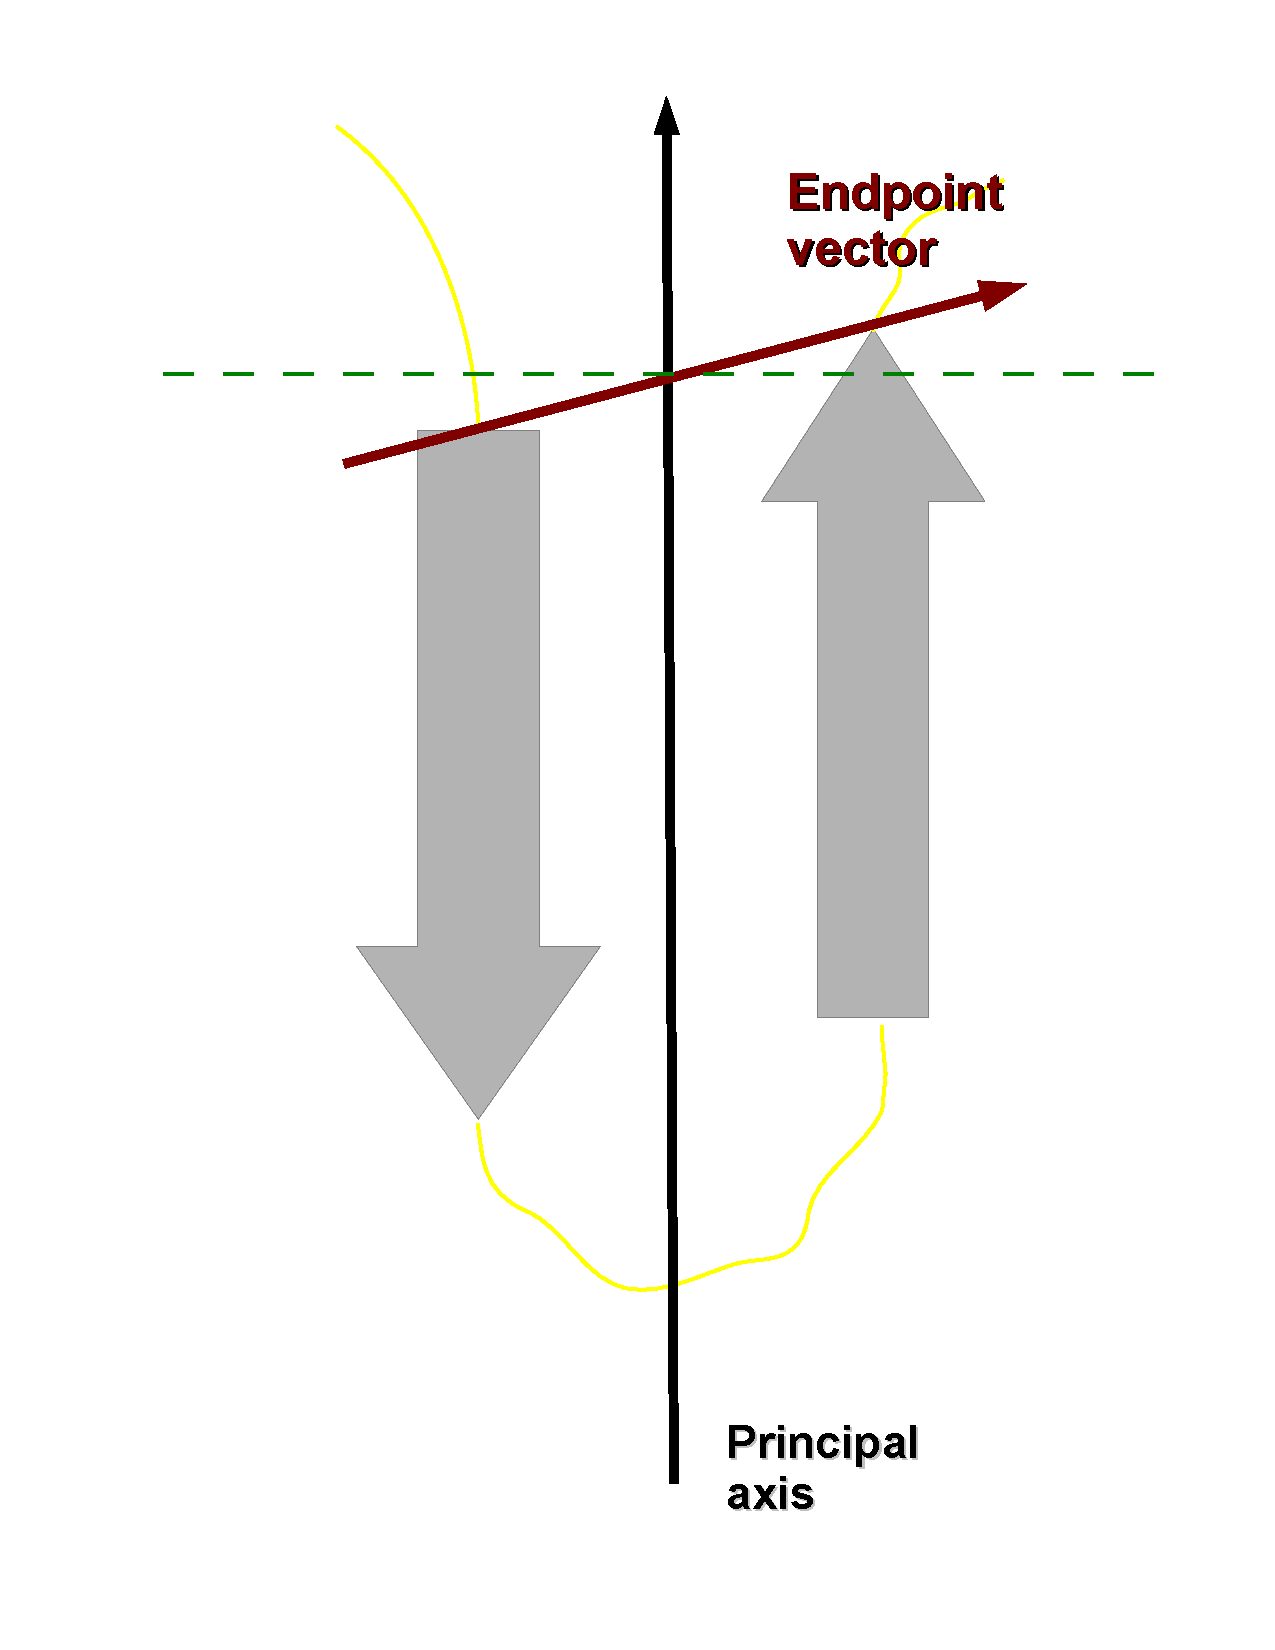
\includegraphics[width=6cm]{images/error-beta-sheet.pdf}
\caption{Litigious case for the orientation of the principal axis. Assume the two $\beta$-strands are selected. Their principal axis is indicated by the black arrow. The red endpoint vector, defined using the first and last atoms of the selection, is roughly orthogonal to the principal axis. If, due to conformational fluctuations of the selection, the endpoint vector's orientation crosses the dashed green line, the orientation of the principal axis will artefactually change.} 
\label{fig:litigious-case-tilt}

\end{figure}

Orientation can be ignored by requesting the \verb!--NOORIENT! keyword; the returned angle is then the absolute value of the minimal angle between the two vectors, and is comprised between 0 and 90 degrees. 

\subsection*{Polar/Azimuthal decomposition}

A Polar/Azimuthal decomposition of the tilt angle can be requested using the \verb!--DEC! keyword. The decomposition allows the user to capture both the radial and azimuthal components of the tilt angle, in a reference coordinate system defined using the \verb!SELEREF! group of atoms. If \verb!--DEC! is requested \verb!SELEREF! and \verb!SELE! are thus no longer equivalent.

First, a $Z$ axis is computed as the principal axis of the \verb!SELEREF!. The $X$ axis is then defined as the projection of the vector joining the centers of mass of \verb!SELEREF! and \verb!SELE! onto the plane orthogonal to $Z$. Finally, the $Y$ axis is defined as $Y = Z \wedge X$. The principal axis $v_1$ of \verb!SELE! is decomposed onto the $X,Y,Z$ basis set:
\begin{itemize}
\item $\theta$ (the \textbf{polar angle}) is defined as the angle made by the projection of $v_1$ onto the $XZ$ plane and the $Z$ axis. It measures the "inward-outward" component of the tilt. 
\item $\varphi$ (the \textbf{azimuthal angle}) is defined as the angle made by the projection of $v_1$ onto the $YZ$ plane and the $Z$ axis. It measures the "lateral" component of the tilt.
\end{itemize}
Note that \verb!--NOORIENT! and \verb!--DEC! are incompatible.\\


\textbf{\large Sample Input}:

\begin{verbatim}
BEGIN tilt
--SELEREF /A/468:482/CA
--SELE    /A/693:703/CA
--DEC
END

\end{verbatim}


\clearpage
\section{Pore dimension of ion channels (HOLE)}

The HOLE module is designed to calculate the radius of the pore of a channel protein along the vector describing the pore. It uses the definition of pore radius and the algorithm proposed by Smart~\textit{et al}~\cite{smart1993pore} and implemented in the HOLE software~\cite{smart1996hole}. The input of the algorithm is a first point located inside the pore, and an approximation of the pore direction. The algorithm first explores the plane perpendicular to the pore axis using a Monte Carlo (MC) approach to find the point where the radius of a sphere non overlapping any atom is maximum. Once it has been found, the current radius is saved, and the point is moved along the pore vector by a specified displacement. The Monte Carlo search is thus performed again in the new plane to find the new biggest sphere radius. The algorithm proceeds moving the point all along the channel vector and the size of the biggest sphere, that is the estimation of the pore radius, is evaluated. The calculation stops when the pore radius is bigger than a threshold value, meaning that the bulk is explored and not anymore the pore of the channel.

As minimal inputs, a point inside the pore \verb#--POINT# and the pore axis \verb#--VECT# are needed (the default values are 0,0,0 for the initial point and 0,0,1 for the axis). Then it is possible to set the maximum pore radius which ends the run (\verb#--RMAX#, default 10\,\AA), and the displacement along the pore axis at each step (\verb#--DISP#, default 0.1\,\AA). To increase the performances of the algorithm a neighbor list is used to speed up the calculation of the maximum sphere radius. This involves the introduction of a cutoff distance (\verb#--CUTOFF#, default 5\,\AA), which is used to build the neighbor list. This cutoff is adaptively changed during the run in order to keep the cutoff small when the pore is narrow, and to increase it when the pore gets wider, but is is assured to be at least as big as the specified \verb#--CUTOFF#. 

In order to tune the Monte Carlo search the following parameters can be changed; note however that the default should be in general good. The first parameter is the seed used in the generation of random numbers (\verb#--SEED#). By default a random seed is used, but a custom seed can be specified to ensure reproducibility of the calculations. Then, the Monte Carlo search consists in the the exploration of the plane perpendicular to the channel vector. A maximum of \verb#--NMAX# steps are performed (default 1000), where each step allows a maximum displacement \verb#--DMAX# (default 0.1\,\AA). The acceptance of a step depends on the new calculated radius: if the radius increases, the move is accepted, if it reduces, it is accepted based on a Boltzmann probability. This introduces the \verb#--KBT# option which determine the acceptance ratio (default for \verb#--KBT# is 0.1\,\AA). Moreover, the ``temperature'' is annealed during the Monte Carlo search, so that \verb#--KBT# is reduced at each step by a scaling factor \verb#--SCALE# (default 0.9). 

The last needed parameter is the van der Waals radius of each atom. These are taken from the historical work of Bondi~\cite{bondi1964vanderwaals}, which are, in angstrom: 1.70 for carbon, 1.52 for oxygen, 1.80 for sulfur, 1.55 for hydrogen, 1.20 for hydrogen, and 1.80 for phosphorus. For all other elements a default radius of 2\,\AA\ is used and a warning is printed. These are, at the moment, hard coded and cannot be changed from command line. Plans are for allowing to read them from an external file in future. 

\clearpage
A summary of all options is here reported:
\begin{longtable}{l|c|p{5.0cm}|l}
\bf{Flag} & \bf{Argument} & \bf{Input} & \bf{Default}\\
\hline\endhead
-{}-TITLE    & string              & Used for output file name                       & pore \\
-{}-POINT    & (float:float:float) & Initial point inside the pore of the protein    & (0:0:0) \\
-{}-VECT     & (float:float:float) & Vector describing the pore axis                 & (0:0:1) \\
-{}-DISP     & float               & Displacement along the pore axis at each step   & 0.1\,\AA\\
-{}-RMAX     & float               & Maximum pore radius which stops the calculation & 10\,\AA\\
-{}-CUTOFF   & float               & Cutoff to update the neighbor list              & 5\,\AA\\
-{}-SEED     & int                 & Seed for the random number generator            & 0 (random seed)\\
-{}-NMAX     & int                 & Number of steps in Monte Carlo search           & 1000\\
-{}-DMAX     & float               & Maximum displacement in Monte Carlo search      & 0.1\,\AA\\
-{}-KBT      & float               & ``Temperature'' used in Monte Carlo search      & 0.1\,\AA\\
-{}-SCALE    & float               & Annealing scaling factor                        & 0.9\\
\end{longtable}

Three output files are generated, which are called based on the \verb#--TITLE# option: \verb#title-prof.dat#, \verb#title-traj.vtf#, and \verb#title-visu.tcl#. The first, \verb#title-prof.dat#, contains the pore radius as a function of the displacement along the channel vector. The format is very accessible via graphing software like gnuplot: in the first column the position along the channel vector is reported, while the pore radius at the frame $N$ can be found in the $N+1$ column. The second file, \verb#title-traj.vtf#, is a trajectory which contains the dynamic of the spheres building up the pore. The use of the VTF file format was needed in order to correctly visualize the sphere sizes in the VMD software. To be able to correctly open the VTF file, the last version of the VTF plugin (2.4) has to be used~\cite{vtfplugin}. The last file in output, \verb#title-visu.tcl#, is a TCL script which can be loaded in VMD to visualize the protein and the pore dynamic together. Due to the variability of the wordom capability of reading trajectories, the TCL script works only in the case where the trajectory is specified as a single file, and no begin, end, or skip options are used. However this TCL script can be modified by hand to handle your specific case. 

\clearpage
\subsection*{Sample Inputs}

Directly from command line:
\begin{verbatim}
wordom -imol 4COF.pdb -itrj 4COF.pdb -ia HOLE --TITLE 4COF \
    --POINT \(3.5:-1.1:139.9\) --VECT \(0.34:0.01:0.94\) --SELE "*" 
\end{verbatim}
Using a wordom script:
\begin{verbatim}
wordom -imol 2VL0.pdb -itrj 2VL0.pdb -iA hole.inp  
\end{verbatim}
Content of \verb#hole.inp#: 
\begin{verbatim}
BEGIN HOLE
--TITLE 2VL0a
--POINT (-104.2:-43.2:-44.4)
--VECT (-0.09:0.22:0.97)
--SELE /@(A|B|C|D|E)///
END
\end{verbatim}
Inside the \verb#test/# directory, it is possible to find some sample inputs and reference outputs. 



\clearpage
\section{Water flux trough a channel (FLUX)}

This module allows to compute the number of molecules (water or ions usually) going through a channel along a trajectory. 

Having as reference Fig.~\ref{fig:flux-scheme}, where the dark gray oval represents the channel, the light gray area an impermeable membrane and all the white the empty space filled of water, a transition is defined as the displacement of a molecule from above the upper boundary to below the lower boundary, going through the channel. 

The algorithm works as follow. All water molecules are given a status, updated every frame. It can be 0, 1, or 3. Only changing from 0 to 1, or 1 to 0, is considered as a true transition. All water molecules contained in the layer defined by the upper boundary and the spacer delta are given the status 0, while all molecules contained in the layer defined by the lower boundary and delta are given the status 1. Other water molecules are given status 3. As the simulation goes, status are updated. If one water molecule with 0 or 1 status moves in the space between the two boundaries, it keeps its previous status. Only when the molecule reaches the other boundary a transition is counted. No distinction is made between the flux going in the upward or the downward direction.

As described, this algorithm assumes the channel is aligned along the $z$ cartesian coordinate, and all atoms have to be be wrapped inside the primary unit cell if periodic boundary conditions (PBC) are used. Please, align and wrap your trajectory before running this module. Moreover, the dynamic of the tracked atoms has to be continuous, so a decent save frequency during the dynamic production is needed. 

\begin{figure}[hb]
  \centering
  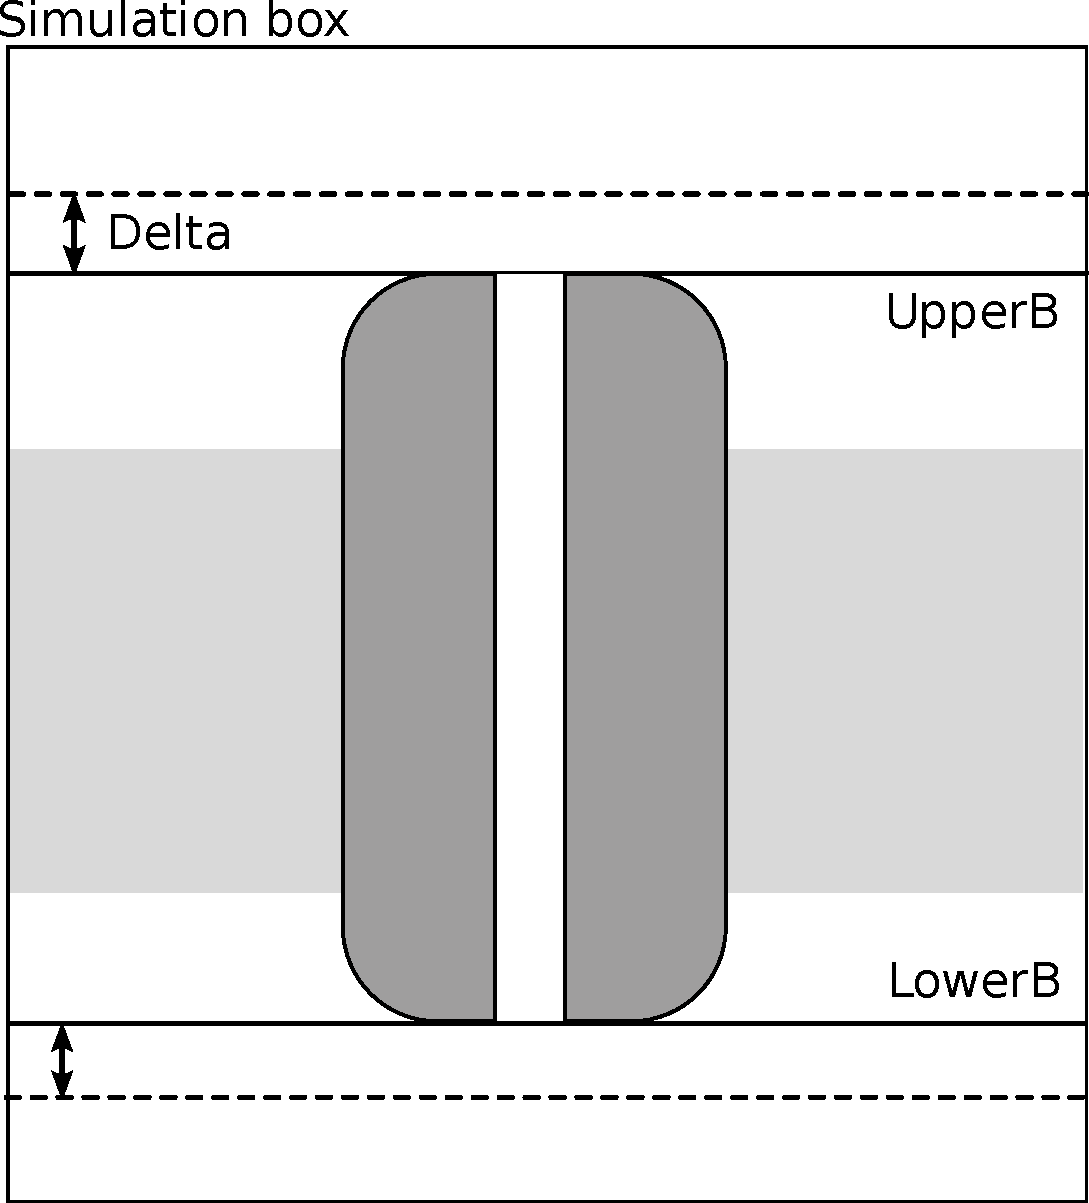
\includegraphics[width=7.0cm]{images/flux-scheme.pdf}
  \caption{Scheme of the definition of upper boundary, lower boundary and delta in the case of a membrane protein.}
  \label{fig:flux-scheme}
\end{figure}

\clearpage
Here a summary of all available options:
\begin{longtable}{l|c|p{6.0cm}|l}
\bf{Flag} & \bf{Argument} & \bf{Input} & \bf{Default}\\
\hline\endhead
-{}-TITLE    & string              & Used for output file name                       & flux \\
-{}-SELE     & string              & Selection for the tracked atoms                 & \verb#/*/*/OH2# \\
-{}-LOWER    & float               & Lower boundary                                  & No default\\ 
-{}-UPPER    & float               & Upper boundary                                  & No default\\ 
-{}-DELTA    & float               & Delta for the two boundaries                    & 5~\AA \\
-{}-REF      & string              & Atoms selection for the channel                 & \verb#/*/*/CA# \\
-{}-RCUT     & float               & Radius of the cylinder in which the transition are taken into account & Not used \\
\end{longtable}

As usual, \verb#--TITLE# species a title for the run, while \verb#--SELE# defines which atoms are tracked along the trajectory; thus if a flux of chlorine ions is wanted \verb#--SELE# should contain something like \verb#/*/*/CL#, while if a water flux is needed the default (\verb#/*/*/OH2#) can be used. As a side note, only one atom per tracked molecule has to be selected, so for water only the oxygen atoms are selected. The \verb#--TITLE# is used as base for an output file called \verb#title-trans.dat#, which contains all the spotted transitions. 

The two options \verb#--LOWER# and \verb#--UPPER# have been already described, together with \verb#--DELTA#, which was created to avoid PBC issues. Indeed, working with PBC, one has to take care of not counting false transition events of water molecules, i.e.\ from the upper part of the box to the lower part of the box through the PBC. To account only for real transitions we define a thin layer of the simulation box (as shown on Fig.~\ref{fig:flux-scheme}) using the upper or lower boundary and a delta value set by default to 5~\AA. All molecules over \verb#--UPPER# plus \verb#--DELTA# or below \verb#--LOWER# minus \verb#--DELTA# are given the undefined status~3. 

The \verb#--REF# and \verb#--RCUT# options were designed so one can be sure the transition spotted occurs inside the channel and not outside of it. A transition is spotted only if the molecule pass thought the channel staying inside a vertical cylinder centered at the center the channel and having radius \verb#--RCUT#. The \verb#--REF# keyword specifies which atoms build the channel, so to define its center. This option can be used, for instance, to remove the few events of transition that could happen through the lipid bilayer in the case of a protein channel embedded in membrane. By default, this option is disabled.

\subsection*{Sample Input}

\begin{verbatim}
BEGIN FLUX
--SELE /*/*/OH2
--LOWER -50.83
--UPPER 2.432
--DELTA 5.0
--RCUT 15.0
END
\end{verbatim}
\verb#wordom -iA flux.inp -imol mol.pdb -itrj traj.dcd -otxt output.out#



% ##################### More Analysis ##################### %

\chapter{More Analyses}
%\addcontentsline{toc}{chapter}{More Analyses}

Although Wordom was conceived to run analysis on trajectory files, i.e., on series of coordinates sets, there are also modules that operate on single structures, small sets of structures or even different kinds of data (usually extracted from trajectories, though).
These modules are called using the -ie/-iE flags, rather than -ia/-iA (as usual, uppercase for input file, lowercase for command line)

\section{Free Energy Basins and Barriers Analysis}

Wordom has two distinct modules, cFEP and KGA, devoted to the identification of (meta)stable states sampled by MD simulations. The key idea of cFEP and KGA is to group conformations not according to structural criteria, but mainly according to equilibrium kinetics.

\subsection{Cut-based free-energy profiles (cFEP)}

The cFEP module refers to a rigorous method introduced by Krivov and Karplus\cite{Krivov:One} for determining a one-dimensional free energy profile that preserves the barriers between free energy basins; given the barriers, free energy basins can be determined. The method uses the relative partition function, which is a reaction coordinate that takes into account all possible pathways to a reference state (e.g., the folded state).

\subsubsection{Pfoldf}

\begin{tabular}{l|c|l|l}
Option & Argument & Input&Default \\
\hline
-ie/BEGIN    & pfoldf & option to call the module &\\
-{}-CLUSFILE & string & timeseries of noderanks & \\
-{}-TEMP     & float  & temperature of the system & 300K \\
-{}-LAMBDA   & float  & Lagrange multiplier & 0.0001 (if target2=0) \\ 
 &&&0 (else) \\
-{}-TARGET   & string & start node (pfold=1) \\
-{}-TARGET2  & string & stop node (node with pfold=0) & 0 (= extra node) \\
-{}-NIT      & int    &  \# of iterations to solve the equations &  50000\\
-{}-NONSYMM  &        &  prevents symmetrization of network & no argument\\
-{}-SYMM     &        &  force symmetrization of network & no argument\\
\end{tabular}\\

\noindent Note that the output file contains nodes sorted according to their weight (number of snapshots). Therefore, to plot the profile it is possible to stop the calculation after a desired number of output pairs and then sort according to column 1 (e.g., $\mid$ head -2000 $\mid$ sort -nk1). The columns in the output file are \$1=$Z_{A}/Z$, \$2=$\Delta{}G$, \$3=$p_{fold}$, \$4=rank of node\\

\noindent By default a nonsymmetrized (detailed balance is not imposed) network is used: detailed balance can be forced by specifying the -{}-SYMM option.\\

\noindent ATTENTION: If pieces of trajectories from different simulations are concatenated, insert a line with the entry ``0'' in between to prevent spurious transitions, i.e., to avoid them to be treated as a continous timeseries. ``0'' must not be used otherwise.\\

{\bf Example:}

\begin{verbatim}wordom -ia pfoldf --CLUSFILE noderank.tt --TARGET 1 --TARGET2 0
 --LAMBDA 0.0001 --NIT 100000 \end{verbatim}

%\vspace{0.25cm}
\subsubsection{Pfoldfnet}

Instead of reading the timeseries of the noderanks, it is also possible to calculate the profile from the linkfile (i.e., the network). Note that this is more efficient than using the option -{}-CLUSFILE.\\

\noindent\begin{tabular}{l|c|l|l}
Option & Argument & Input & Default \\
\hline
-ie/BEGIN    & pfoldfnet & option to call the module\\
-{}-LINKFILE & string & links and weights (three-column file)\\
-{}-TEMP     & float  & temperature of the system & 300K \\
-{}-LAMBDA   & float  & Lagrange multiplier & 0.0001 (if target2=0) \\ 
 &&&0 (else) \\
-{}-TARGET   & string & start node (pfold=1) \\
-{}-TARGET2  & string & stop node (node with pfold=0) & 0 (= extra node) \\
-{}-NIT      & int    &  \# of iterations to solve the equations &  50000\\
-{}-NONSYMM  &        &  prevents symmetrization of network & no argument\\
-{}-SYMM     &        &  force symmetrization of network & no argument\\
\end{tabular}\\

\noindent The output format is identical to the one from the pfoldf function.\\


{\bf Example:}

\begin{verbatim}wordom -ie pfoldfnet --LINKFILE linkfile.txt --TARGET 1 --TARGET2 0
 --LAMBDA 0.0001 \end{verbatim}


%\vspace{0.25cm}
\subsubsection{Mfpt}

\noindent\begin{tabular}{l|c|l|l}
Option & Argument & Input & Default \\
\hline
-ie/BEGIN    & mfpt & option to call the module &\\
-{}-CLUSFILE & string & timeseries of noderanks &\\
-{}-TEMP     & float  & temperature of the system & 300K \\
-{}-TARGET   & string & start node (pfold=1) \\
-{}-NIT      & int    & \# of iterations to solve the equations & 50000\\
-{}-NONSYMM  &        &  prevents symmetrization of network & no argument\\
-{}-SYMM     &        &  force symmetrization of network & no argument\\
\end{tabular}\\

\noindent As for pfoldf, the output file contains nodes sorted according to their weight (number of snapshots). Therefore, to plot the profile it is possible to stop the calculation after a desired number of output pairs and then sort according to column 1 (e.g., $\mid$ head -2000 $\mid$ sort -nk1). To use mfpt as reaction coordinate instead of $Z_{A}/Z$: the columns in the output file are \$1=$Z_{A}/Z$, \$2=$\Delta{}G$, \$3=mfpt, \$4=rank of node. Therefore, (x=\$1,y=\$2) is the usual $\Delta{}G$ vs. $Z_{A}/Z$ plot, while (x=\$3, y=\$2) is the $\Delta{}G$ vs. mfpt plot, where the separation from the target basin is measured by a distance in time units.\\

\noindent By default a nonsymmetrized (detailed balance is not imposed) network is used: detailed balance can be forced by specifying the -{}-SYMM option.\\

\noindent ATTENTION: If pieces of trajectories from different simulations are concatenated, insert a line with the entry ``0'' in between to prevent spurious transitions, i.e., to avoid them to be treated as a continous timeseries. ``0'' must not be used otherwise.\\

{\bf Example:}

\begin{verbatim}wordom -ie mfpt --CLUSFILE noderank.tt --TARGET 1  --NIT 100000 
--NONSYMM --TEMP 330 \end{verbatim}


%\vspace{0.25cm}
\subsubsection{Mfptnet}

In analogy to the pfoldfnet function, also mfpt profiles can be calculated by giving the linkfile as input. This is more efficient than using the clusfile.\\

\noindent\begin{tabular}{l|c|l|l}
Option & Argument & Input & Default \\
\hline
-ie/BEGIN    & mfptnet& option to call the module\\
-{}-LINKFILE & string & links and weights (three-column file) \\
-{}-TEMP     & float  & temperature of the system & 300K \\
-{}-TARGET   & string & start node (pfold=1) \\
-{}-NIT      & int    & \# of iterations to solve the equations & 50000\\
-{}-NONSYMM  &       &  prevents symmetrization of network & no argument\\
-{}-SYMM     &        &  force symmetrization of network & no argument\\
\end{tabular}\\
\vspace{3mm}

{\bf Example:}

\begin{verbatim}wordom -ie mfptnet --LINKFILE linkfile.txt --TARGET 1  --TEMP 330 \end{verbatim}
\subsection{KGA}
Two microstates are grouped if along the MD trajectory their snapshots interconvert in more than 50\% of the cases within a short commitment time $\tau_{commit}$, which represents a typical relaxation time within basins of the investigated system~\cite{Muff:Kinetic}. The idea behind this approach is that if two conformations interconvert rapidly, they are not separated by a barrier and therefore belong to the same basin. Microstates are first defined with a clustering of MD snapshots according to geometrical criteria (RMSD) or based on properties such as secondary structure.

\subsubsection{logbin module: First passage time - plot to find $\tau_{commit}$}

Reads in the timeseries of noderanks (i.e., a one-column file, each row indicating the rank of the population of the node, e.g., most populated node=1, second most populated node=2, etc.) and gives back the x- and y-coordinates of the logarithmically binned free-energy fpt-plot with respect to a selected node.\\

\begin{tabular}{l|c|l}
Option & Argument & Input \\
\hline
-ie/BEGIN		 & logbin & option to call the logbin module\\
-{}-CLUSFILE & string & timeseries of noderanks \\
-{}-BPD      & int    & bins per decade \\
-{}-TARGET   & int    & nodename with respect to which the first passage \\
 & & time should be calculated \\
\end{tabular}\\
\\

{\bf Example:}

\begin{verbatim}wordom -ie logbin --CLUSFILE noderank.tt --BPD 10 --TARGET 1 \end{verbatim}

%\vspace{0.25cm}
\subsubsection{ka module: Kinetic grouping analysis to isolate all basins at once}

Reads in the timeseries of noderanks and groups nodes into basins according to KGA. The procedure calculates the all-against-all matrix for a selected number of most populated nodes and assigns all other nodes in a postprocessing step.\\

\begin{tabular}{l|c|l}
Option & Argument & Input \\
\hline
-ie/BEGIN 	 & ka & option to call the KGA module\\
-{}-CLUSFILE & string & timeseries of noderanks \\
-{}-TCOMM    & int    & commitment time $\tau_{commit}$ (number of frames) \\
-{}-NNODES   & int    & number of nodes for all-against-all \\
\end{tabular}\\
\\

{\bf Example:}

\begin{verbatim}wordom -ie ka --CLUSFILE noderank.tt --TCOMM 50 --NNODES 500 \end{verbatim}

%\vspace{0.25cm}
\subsubsection{basin module: Kinetic grouping analysis to isolate a single basin}

Reads in the timeseries of noderanks. The output is the list of commitment probabilities ($p_{commit}$) of all nodes to the target node. The last part of the output is a list of all nodes in the basin of the selected targetnode.\\

\begin{tabular}{l|c|l}
Option & Argument & Input \\
\hline
-ie/BEGIN    & basin & option to call the basin isolation module\\
-{}-CLUSFILE & string & timeseries of noderanks \\
-{}-TCOMM    & int    & commitment time $\tau_{commit}$ (number of frames) \\
-{}-TARGET   & int    & nodename (rank) of the target node\\
\end{tabular}\\
\\

{\bf Example:}
 
\begin{verbatim}wordom -ie basin --CLUSFILE noderank.tt --TCOMM 50 --TARGET 1 \end{verbatim}


%\vspace{0.25cm}

\subsection{A posteriori equilibration of out of equilibrium simulations}

(Experimental: use at your own risk) For many systems long equilibrium simulations are unfeasible. Therefore, the focus is often put on the sampling of transitions following only one direction, starting in regions of relatively high energy and terminating once the system reaches the low-energy region of interest (e.g., the folded state). The result is an ensemble of out of equilibrium (kinetic) simulations, which do not represent a thermodynamically correct picture of the free-energy surface. The low-energy state will remain underrepresented, because the simulation time-scale is much shorter than the expected unfolding time.

Despite the incorrect overall thermodynamic picture, it can be assumed that locally the transition probabilities ($p_{ij}=n_{ij}/n_{j}$ to go from node j to i within one time step, given that the trajectory is currently in j) are correct. By solving the system of equations, corresponding to the correct population probabilities $p_{i}^{eq}$ of the nodes, new weights are assigned to all nodes and links.
The system of equations
%
\begin{eqnarray*}
p_i^{eq} &=& \sum_{j}{p_{ij}} \cdot p_j^{eq} \\ 
\sum_{i} {p_i^{eq}}& =&1
\end{eqnarray*}
is used to ``equilibrate'' the weights of the nodes (where $n_j^{eq}=p_j^{eq} N$, with $N$ being the total number of snapshots in the trajectory).
%
The weights of the links are then ``equilibrated'' by
%
\begin{eqnarray*}
n_{ij}^{eq}=p_{ij}\cdot n_j^{eq} \ .
\end{eqnarray*} 
%

\begin{tabular}{l|c|l|l}
Option & Argument & Input & Default \\
\hline
-ie/BEGIN    & equil & option to call the module\\
-{}-LINKFILE & string & links and weights (three-column file) \\
-{}-NIT      & int    & \# of iterations to solve the equations & 100'000\\
\end{tabular}\\\vspace{5mm}


{\bf Example:}

\begin{verbatim}wordom -ie equil --LINKFILE linkfile.txt  --NIT 80000 \end{verbatim}

\clearpage

\section{Ring Perception Module (RING)}

The RING Module for WORDOM performs a ring search using the ring perception algorithm proposed by Hanser et al.\cite{hanser}. The main idea is to find supramolecular cyclic structures, for example hexagons or other polygons, but the algorithm is quite generic and can be used for any ring perception problem. 
	
The input file consists essentially in a graph in a very simple format: a set of lines, each one containing two numbers. These numbers are the id of an object (could be an atom or a molecule, or whatever you want), and each line means that the two objects identified by the two numbers are in contact. A sample graph file for a pentagon needs only the following lines:

\begin{verbatim}
  1 2
  2 3
  3 4
  4 5
  5 1
\end{verbatim}
Very important, each contact must be present only once and duplicates {\em eg} \verb=1 2= and \verb=2 1= must not be present. If you want to analyse only one graph file your wordom input file is simply:

\begin{verbatim}
BEGIN RING
--GRAPH mygraph.inp
END
\end{verbatim}

You can specify two optional parameters: \verb=RINGS= and \verb=DIM=. \verb=RINGS= allow you to specify an output file where the perceived rings are saved, the default name being \verb=rings.dat=. The format of this output is quite simple: the first column contains the dimension of the ring and the following columns contain the id of each object that builds that ring. The parameter \verb=DIM= is very useful when you have a lot of condensed rings. In this case a full ring search will find a large number of rings. With the \verb=DIM= parameter only the rings with a dimension less than \verb=DIM= will be saved and printed. The default value for \verb=DIM= is 10. A complete wordom input file if we are interested only in polygons up to hexagons could be:

\begin{verbatim}
BEGIN RING
--GRAPH mygraph.inp
--RINGS myroutput.dat
--DIM 6
END
\end{verbatim}
%
or directly via command line:

\begin{verbatim}
wordom -ie RING --GRAPH mygraph.inp --RINGS myoutput.dat --DIM 6
\end{verbatim}

A second way to use this module is via the \verb=LIST= parameter which is useful if you need to analyse a lot of graphs. In such case you only need to save each graph in a separate file, and then put all file names in a list file one per line, for example:

\begin{verbatim}
mygraph1.inp
graph2.inp
mythirdgraph.inp
finalgraph.inp
\end{verbatim}
%
Then you can run wordom like:

\begin{verbatim}
BEGIN RING
--LIST mygraphlist.inp
--RINGS myroutput.dat
--DIM 6
END
\end{verbatim}
%
The \verb=GRAPH= and \verb=LIST= options are obviously mutually exclusive.

There is a last parameter you can use: \verb=STATS=. If you specify this parameter followed by an output file name, the module will make a statistics about ring dimension for each analysed graph and will print the result in the specified output file. This is interesting, for example, when the graphs are representative of the frames of a trajectory, so you will obtain the statistics of the formed rings along the trajectory. The format of this file is: in the first column a number indicating the input file, and then a list of number indicating the frequency of cycles at each dimension: so in the second column you will find the number of cycle with dimension 1 (always zero), in the third column with dimension two (always zero), in the fourth column the triangles, and so on.

Finally, \verb=--HELP= will print this help and \verb=--VERSION= will print version number and copyright of the current RING Module for WORDOM.

\paragraph*{Usage:}
\verb=wordom -ie RING [OPTION]...=\\


\textbf{\large Options}:\\\\
\begin{tabular}{l|c|p{7.0cm}}
Flag & Argument & Input \\
\hline
\verb=--GRAPH=    & filename      & input file name (single graph)\\
\verb=--LIST=     & filename      & input file name (list of graphs)\\
\verb=--DIM=      & int           & maximum size of rings; bigger rings are ingored; default 10\\
\verb=--RINGS=    & filename      & output file name for the list of detected rings; default is \verb=rings.dat=\\
\verb=--STATS=    & filename      & output file name for ring size statistics; if not set no statistics are performed\\
\verb=--HELP=     & none          & show this help and exit\\
\verb=--VERSION=  & none          & print version information and exit\\
\end{tabular}\\\\

%\paragraph*{Options:}
%\begin{itemize}
	%\item \verb=--GRAPH=: input file name (if analysing a single graph)
	%\item \verb=--LIST=: input file name (if analysing a list of graphs)
	%\item \verb=--DIM=: the maximum dimension of rings; bigger rings are not perceived; default 10
	%\item \verb=--RINGS=: output file name for the list of perceived rings; default is \verb=rings.dat=
	%\item \verb=--STATS=: output file name for ring dimension statistics; if not set no statistics are performed
	%\item \verb=--HELP=: show this help and exit
	%\item \verb=--VERSION=: print version information and exit
%\end{itemize}

\paragraph*{Examples:}

Analyse only a graph in \verb=mygraph.dat= file and outputs the perceived rings in \verb=rings.dat=. No statistics are performed on ring dimension. Use the default dimension of 10 for maximum ring dimension.

\begin{verbatim}
wordom -ie RING --GRAPH mygraph.dat --RINGS rings.dat
\end{verbatim}


Analyse all graphs listed in \verb=mylist.dat=, save all perceived rings in \verb=rings.dat= and save a statistic of rings dimension along all graphs in \verb=stats.dat=. Perceive only rings smaller than a pentagon.

\begin{verbatim}
wordom -ie RING --LIST mylist.dat --RINGS rings.dat \
       --STATS stats.dat --DIM 5
\end{verbatim}

\clearpage






%\chapter{PyWordom}
%\section{Installation}
%The basic IO functions of Wordom have been wrapped with the SWIG\cite{Beazley:SWIG} tool into a python module.\\
%Since the pywordom module is not pure python but has a compiled C core it must be recompiled, too. To recompile just go to the sources directory and type:
%\begin{verbatim}
%python setup.py build
%\end{verbatim}
%Then, as root, run the command:
%\begin{verbatim}
%python setup.py install
%\end{verbatim}
%This will install the wordom python module in system directories. The {\em import wordom} line in a python script will include the wordom module.
%\begin{verbatim}
%#!/bin/env python
%import wordom as wrd
%\end{verbatim}


%\section{Usage}
%The {\em wordom} python module allows simple python scripts to access data in the pdb, crd, dcd and xtc formats. Most of the available functionalities are provided through the {\em molecule}, {\em trajectory}, {\em coordinates} and {\em selection} objects:

%Create a new instance of the Molecule class:\\
%mol1 = wrd.NewMolecule()

%destroy a molecule instance:\\
%wrd.DesMolecule(mol1)

%create a selection instance:\\
%sele1 = wrd.NewSele()

%create a trajectory instance:\\
%trj1 = wrd.NewTraj()

%destroy a trajectory instance:\\
%wrd.DesTrajtrj1)

%create a trajectory header instance:\\
%trh1 = wrd.NewTrjh()

%create a coordinates set instance:\\
%coor1 = wrd.NewCoor()

%destroy a coordinates set instance:\\
%wrd.DesCoor(coor1)

%Functions and methods to play with these structure:

%Accessing $nn^{th}$ coordinate inside a coordinate set:\\
%coor1.x(nn)\\
%coor1.y(nn)\\
%coor1.z(nn)

%Setting $nn^{th}$ coordinate inside a coordinate set:\\
%coor1.setx(nn, xvalue)\\
%coor1.sety(nn, yvalue)\\
%coor1.setz(nn, zvalue)\\
%coor1.setcoor(nn, xvalue, yvalue, zvalue)\\

%Copying values from another coordinate set:\\
%coor1.copycoor(coorset2)\\

%Extract a subset of coordinates:\\
%subset1 = coor.getselecoor( sele1 )\\

%-\\

%{\bf Example:}
%\begin{verbatim}
%import wordom as wrd

%mymol = wrd.Molecule()
%mymol.read( "./structure.pdb" )
%mymol.write( "./copy.pdb" )

%sele1 = mymol.select( "/CA" )
%print sele1.nselatm
%mymol2 = mymol.getselemol(sele1)
%mymol2.write( "submol.pdb" )

%\end{verbatim}

%Classes:
%Molecule


%Methods:

\begin{thebibliography}{10}
\addcontentsline{toc}{chapter}{Bibliography}

\bibitem{mseeber:wordom}
M.~Seeber, M.~Cecchini, F.~Rao, G.~Settanni, and A.~Caflisch, {\em
  Bioinformatics}, {\bf 2007}, {\em 23}(19), 2625--2627.

\bibitem{mseeber:wordom2}
M.~Seeber, A.~Felline, F.~Raimondi, S.~Muff, R.~Friedman, F.~Rao, A.~Caflisch,
  and F.~Fanelli, {\em J. Comp. Chem}, {\bf 2010}, in press.

\bibitem{baybren}
http://dx.doi.org/10.1080/2151237X.2008.10129266

\bibitem{cecchini:amyloid}
M.~Cecchini, F.~Rao, M.~Seeber, and A.~Caflisch, {\em J. Chem. Phys.}, {\bf
  2004}, {\em 121}.

\bibitem{2001JChPh.115.6289A}
I.~{Andricioaei} and M.~{Karplus}, {\em J. Chem. Phys.}, {\bf 2001}, {\em 115},
  6289--6292.

\bibitem{DSSP}
W.~Kabsch and C.~Sander, {\em Biopolymers}, {\bf 1983}, {\em 22}(12),
  2577--637.

\bibitem{DSSP:cont1}
C.~A.~F. Andersen, A.~G. Palmer, S.~Brunak, and B.~Rost, {\em Structure}, {\bf
  2002}, {\em 10}, 174--184.

\bibitem{DSSP:cont2}
P.~Carter, C.A.F. Andersen, and B.~Rost, {\em Nucleic Acids Research}, {\bf
  2003}, {\em 31}(13), 3293.

\bibitem{tirion:96}
Tirion, M., {\em Phys Rev Lett}, 1996, {\bf 77}(9), 1905--1908.

\bibitem{delarue:2002}
Delarue, M. and Sanejouand, Y., {\em J Mol Biol}, 2002, {\bf 320}(5),
  1011--1024.

\bibitem{kovacs:ppf}
Kovacs, J., Chac{\'o}n, P. and Abagyan, R., {\em Proteins}, 2004, {\bf 56}(4),
  661--668.

\bibitem{Durand:1994}
Durand, P., Trinquier, G. and Sanejouand, Y.-H., {\em Biopolymers}, 1994, 34, 759−771.

\bibitem{Tama:2000}
Tama, F., Gadea, F. X., Marques, O. and Sanejouand, Y. H., {\em Proteins}, 2000, 41, 1−7

\bibitem{Zheng:2005a}
Zheng, W. and Brooks, B. R, {\em Biophys. J.}, 2005, 89, 167−178.

\bibitem{Zheng:2005b}
Zheng,W., Brooks, B., Doniach, S. and Thirumalai, {\em D. Structure}, 2005, 13,565.

\bibitem{Wang:2004}
Wang, Y., Rader, A. J., Bahar, I. and Jernigan, R. L, {\em J. Struct. Biol.}, 2004, 147, 302−314.

\bibitem{buvsa2005afp}
J.~Bu{\v{s}}a, J.~D{\v{z}}urina, E.~Hayryan, S.~Hayryan, C.K. Hu, J.~Plavka,
  I.~Pokorn{\`y}, J.~Sk{\v{r}}iv{\'a}nek, and M.C. Wu, {\em Computer Physics
  Communications}, {\bf 2005}, {\em 165}(1), 59--96.

\bibitem{pascualahuir1994gid}
JL~Pascual-Ahuir, E.~Silla, and I.~Tunon, {\em Journal of Computational
  Chemistry}, {\bf 1994}, {\em 15}(10).

\bibitem{mccammon1988dynamics}
J.A. McCammon and S.C. Harvey, {\em {Dynamics of proteins and nucleic acids};}
\newblock Cambridge Univ Pr, 1988.

\bibitem{kraskov2004estimating}
A.~Kraskov, H.~Stoegbauer, and P.~Grassberger, {\em Physical Review E}, {\bf
  2004}, {\em 69}(6), 66138.

\bibitem{lange2006generalized}
O.F. Lange and H.~Grubmuller, {\em PROTEINS-NEW YORK-}, {\bf 2006}, {\em
  62}(4), 1053.

\bibitem{brinda05}
K.~V. Brinda and S.~Vishveshwara, {\em Biophys. J.}, {\bf 2005}, {\em 89},
  4159--4170.

\bibitem{ghosh2007study}
A.~Ghosh and S.~Vishveshwara, {\em Proceedings of the National Academy of
  Sciences}, {\bf 2007}, {\em 104}(40), 15711.

\bibitem{Krivov:One}
S.~V. Krivov and M.~Karplus, {\em J. Phys. Chem. B}, {\bf 2006}, {\em 110},
  12689--12698.

\bibitem{Muff:Kinetic}
S.~Muff and A.~Caflisch, {\em Proteins: Structure, Function, and
  Bioinformatics}, {\bf 2008}, {\em 70}, 1185--1195.

\bibitem{hanser}
Hanser et al., {\em J. Chem. Inf. Comput. Sci.}, {\bf 1996}, {\em 36} (6), 1146--1152 DOI:10.1021/ci960322f

\bibitem{Beazley:SWIG}
D. Beazley, {\em The Simple Wrapper and Interface Generator}. Available at: \url{http://www.swig.org}

\bibitem{smart1993pore}
O. S. Smart, J. M. Goodfellow, and B. A. Wallace, {\em Biophysical Journal}, {\bf 1993}, {\em 65}, 2455--2460.

\bibitem{smart1996hole}
O. S. Smart, J. G. Neduvelil, X. Wang, B. A. Wallace, and M. S. P. Sansom, {\em Journal of Molecular Graphics}, {\bf 1996}, {\em 14}, 354--360.

\bibitem{bondi1964vanderwaals}
A. Bondi, {\em Journal of Physical Chemistry}, {\bf 1964}, {\em 68}, 441--451.

\bibitem{vtfplugin}
O. Lenz, {\em VTF Plugin}. Available at: \url{https://github.com/olenz/vtfplugin}


\end{thebibliography}

\clearpage

% ##################### That's All Folks! ##################### %

\end{document}

